\documentclass[11pt]{article}
\usepackage{amsmath}
\usepackage{amsfonts}
\usepackage[body={6.25in,8.85in}]{geometry}
\usepackage{url}
\usepackage[scaled]{helvet}
\usepackage[authoryear,round]{natbib}
\usepackage{graphicx}
\usepackage{rotating}
\usepackage{multirow}
\usepackage{tabularx}
\usepackage{authblk}
\usepackage{xcolor}
\usepackage{changebar}
\usepackage[
  bookmarks=false,
  pdfpagelabels=false,
  hyperfootnotes=false,
  hyperindex=false,
  pageanchor=false,
  colorlinks,
  linkcolor=blue,
  urlcolor=black, 
  citecolor=black
]{hyperref}
\usepackage[singlelinecheck=false]{caption}
\newcommand{\removed}[1]{\cbstart\removedfragile{#1}\cbend{}}
\newcommand{\removedfragile}[1]{{\color{red}{#1}}{}}
\newcommand{\added}[1]{\cbstart\addedfragile{#1}\cbend{}}
\newcommand{\addedfragile}[1]{{\color{red!50!black}{#1}}{}}
\newcommand{\changed}[2]{\protect\added{#1}\protect\removed{#2}}

\setcounter{secnumdepth}{5}

\begin{document}
\title{\textbf{Supplement materials for: Addressing DNase-seq cleavage bias and residence time on computational footprinting}} \date{}

\author[1,2]{Eduardo G. Gusmao}
\author[1,2]{Martin Zenke}
\author[1,2,3]{Ivan G. Costa\thanks{ivan.costa@rwth-aachen.de}}
\affil[1]{IZKF Computational Biology Research Group, RWTH Aachen University Medical School, Aachen, Germany.}
\affil[2]{Department of Cell Biology, Institute of Biomedical Engineering, RWTH Aachen University Medical School, Aachen, Germany.}
\affil[3]{Aachen Institute for Advanced Study in Computational Engineering Science (AICES), RWTH Aachen University, Aachen, Germany.}

\thispagestyle{empty}

\maketitle

\setlength{\parskip}{0.5cm}

\begin{table*}[h!]
\small
\begin{flushleft}
\caption*{\textbf{{\small Supplementary Methods}}}
\vspace{-0.4cm}
\end{flushleft}
\begin{center}
\renewcommand{\arraystretch}{1.2}
\begin{tabularx}{\textwidth}{ |>{\hsize=.1\hsize}X|>{\hsize=.85\hsize}X|>{\hsize=.05\hsize}X| }
\hline
\textbf{Section} & \textbf{Title} & \textbf{Page} \\
\hline
\ref{sec:data} & Data  & \pageref{sec:data} \\
\hline
\ref{sec:cleavage-bias} & Bias Correction  & \pageref{sec:cleavage-bias} \\
\hline
\ref{sec:signal} & DNase I Hypersensitive Sites  & \pageref{sec:signal} \\
\hline
\ref{sec:bias-estimation} & Estimation of DNase I Cleavage Bias  & \pageref{sec:bias-estimation} \\
\hline
\ref{sec:bias-correction} & DNase I Cleavage Bias Correction  & \pageref{sec:bias-correction} \\
\hline
\ref{sec:fp-methods} & Computational Footprinting Methods (in Chronological Order)  & \pageref{sec:fp-methods} \\
\hline
\ref{sec:neph} & Neph Method  & \pageref{sec:neph} \\
\hline
\ref{sec:boyle} & Boyle Method  & \pageref{sec:boyle} \\
\hline
\ref{sec:centipede} & Centipede  & \pageref{sec:centipede} \\
\hline
\ref{sec:cuellar} & Cuellar Method  & \pageref{sec:cuellar} \\
\hline
\ref{sec:wellington} & Wellington  & \pageref{sec:wellington} \\
\hline
\ref{sec:piq} & Protein Interaction Quantification (PIQ)  & \pageref{sec:piq} \\
\hline
\ref{sec:flr} & Footprint Mixture (FLR)  & \pageref{sec:flr} \\
\hline
\ref{sec:dnase2tf} & DNase2TF  & \pageref{sec:dnase2tf} \\
\hline
\ref{sec:hint} & HINT, HINT-BC, HINT-BCN  & \pageref{sec:hint} \\
\hline
\ref{sec:fs} & Footprint Score (FS)  & \pageref{sec:fs} \\
\hline
\ref{sec:tc} & Tag Count (TC)  & \pageref{sec:tc} \\
\hline
\ref{sec:evaluation} & Evaluation  & \pageref{sec:evaluation} \\
\hline
\ref{sec:mpbs} & Motif-Predicted Binding Sites (MPBSs)  & \pageref{sec:mpbs} \\
\hline
\ref{sec:performeval} & Method Comparison  & \pageref{sec:performeval} \\
\hline
\ref{sec:stat-methods} & Statistical Methods  & \pageref{sec:stat-methods} \\
\hline
\ref{sec:protection} & Protection Score  & \pageref{sec:protection} \\
\hline
\end{tabularx}
\end{center}
\end{table*}

\clearpage

\begin{table*}[h!]
\small
\begin{flushleft}
\caption*{\textbf{{\small Supplementary Figures}}}
\vspace{-0.4cm}
\end{flushleft}
\begin{center}
\renewcommand{\arraystretch}{1.2}
\begin{tabularx}{\textwidth}{ |>{\hsize=.25\hsize}X|>{\hsize=.7\hsize}X|>{\hsize=.05\hsize}X| }
\hline
\textbf{Item} & \textbf{Descriptive Title} & \textbf{Page}  \\
\hline
Supplementary Fig.~\ref{fig:tcbiasuwk} & Correlation between the performance of methods and their OBS on {\tt He Dataset} & \pageref{fig:tcbiasuwk} \\
\hline
Supplementary Fig.~\ref{fig:lineOBCsignal} & Average DNase-seq signals around selected TFs with ChIP-seq evidence in H1-hESC (DU) cell type & \pageref{fig:lineOBCsignal} \\
\hline
Supplementary Fig.~\ref{fig:datasetcorr} & Ward's minimum variance clustering on pairwise Spearman correlation coefficient ($R$) between different DNase-seq data sets & \pageref{fig:datasetcorr} \\
\hline
Supplementary Fig.~\ref{fig:bias_cg} & Association between k-mer CG content and cleavage bias & \pageref{fig:bias_cg} \\
\hline
Supplementary Fig.~\ref{fig:auc_boxplot} & AUC distribution for 14 footprinting methods regarding all validation sets (ordered by median AUC) & \pageref{fig:auc_boxplot} \\
\hline
Supplementary Fig.~\ref{fig:lineOBCsignal2} & Average DNase-seq signals around nuclear receptor TFs with ChIP-seq evidence in LNCaP(DU), m3134(UW) and MCF-7(DU) cell types & \pageref{fig:lineOBCsignal2} \\
\hline
Supplementary Fig.~\ref{fig:denovo} & Average bias and DNase-seq signals around binding sites of \emph{de novo} motifs 0458 and 0500 on cell type H7-hESC & \pageref{fig:denovo} \\
\hline
\end{tabularx}
\end{center}
\end{table*}

\begin{table*}[h!]
\small
\begin{flushleft}
\caption*{\textbf{{\small Supplementary Tables}}}
\vspace{-0.4cm}
\end{flushleft}
\begin{center}
\renewcommand{\arraystretch}{1.2}
\begin{tabularx}{\textwidth}{ |>{\hsize=.25\hsize}X|>{\hsize=.7\hsize}X|>{\hsize=.05\hsize}X| }
\hline
\textbf{Item} & \textbf{Descriptive Title} & \textbf{Page} \\
\hline
Supplementary Table~\ref{tab:dataencode} & Summary of DNase-seq data & \pageref{tab:dataencode} \\
\hline
Supplementary Table~\ref{tab:summary} & Summary of computational footprinting methods & \pageref{tab:summary} \\
\hline
Supplementary Table~\ref{tab:fn.table} & Friedman-Nemenyi hypothesis test results on AUC for all evaluated methods & \pageref{tab:fn.table} \\
\hline
\end{tabularx}
\end{center}
\end{table*}

\clearpage

\section{Methods}
\label{sec:methods}

\subsection{Data}
\label{sec:data}

{\color{red!50!black}{
DNase-seq aligned reads were obtained from ENCODE~\citep{encode2012}. We obtained data regarding cell types H1-hESC, HeLa-S3, HepG2, Huvec, K562, LNCaP and MCF-7 from Crawford's Lab (labeled with the initials of their institution ``DU'') and concerning cell types H7-hESC, HepG2, Huvec, K562 and m3134 from Stamatoyannopoulous' lab (labeled with the initials of their institution ``UW''). We also used deproteinized DNase-seq experiments from cell types MCF-7 and K562 (Crawford lab)~\citep{yardimci2014} and IMR90 (Stamatoyannopoulous lab)~\citep{lazarovici2013}. DNase-seq experiments labeled with ``DU'' follow the single-hit protocol, while the experiments labeled with ``UW'' follow the double-hit protocol. See Supplementary Table~\ref{tab:dataencode} for data description.

Transcription factor (TF) ChIP-seq enriched regions (peaks and summits) were obtained in ENCODE Analysis Working Group (AWG) track with exception of the following experiments, in which the enriched regions were obtained using bowtie-2~\citep{langmead2012} and MACS~\citep{zhang2008}. AR (R1881 treatment) ChIP-seq raw sequences for LNCaP cell type was obtained in Gene Expression Omnibus (GEO) with accession number GSM353644~\citep{yu2010}. ER (40 and 160 minutes after estradiol treatment) ChIP-seq raw sequences for MCF-7 cell type was obtained in GEO with accession number GSE54855~\citep{guertin2014}. GR (dexamethasone treatment) ChIP-seq raw sequences for m3134 cell type was obtained in SRA under study number SRP004871~\citep{john2011}. All organism-specific data (DNase-seq and ChIP-seq) are based on the human genome build 37 (hg19), except the DNase-seq for m3134 and ChIP-seq for GR, which were based on mouse genome build 37 (mm9). Chromosome Y was removed from all analyses.

TF motifs (position frequency matrices; PFMs) were obtained from the Jaspar~\citep{mathelier2014}, Uniprobe~\citep{robasky2011} and Transfac~\citep{matys2006} repositories. Non-organism-specific data (PFMs) were obtained for the subphylum Vertebrata. \emph{de novo} PFMs 0458 and 0500 were downloaded from \url{ftp://ftp.ebi.ac.uk/pub/databases/ensembl/encode/supplementary/integration_data_jan2011/byDataType/footprints/jan2011/de.novo.pwm} \citep{neph2012a}. The accession codes for all TF ChIP-seq experiments and PFM IDs are available in the Supplementary Dataset~1.
}}

\subsection{Bias Correction}
\label{sec:cleavage-bias}

\subsubsection{DNase I Hypersensitive Sites}
\label{sec:signal}

A first task is the identification of DNase I Hypersensitivity sites (DHSs). A nucleotide-resolution genome-wide signal was created for each DNase-seq data set by counting reads mapped to the genome. Here, we considered only the 5$^\prime$ position of the aligned reads (position at which DNase I cleaved the DNA). The genomic signal was created by counting the number of reads that overlapped at each genomic position.

More formally, we define a raw genomic signal as a vector
\begin{align*}
  \mathbf{x} = \langle{x}_{1},...,{x}_{N}\rangle,
\end{align*}
where~$N$ equals the number of bases in the genome and each ${x}_{i} \in \mathbb{N}^0$ is the number of DNase-seq reads mapped to position $i$. We also generate strand specific counts $X^s$, where $s \in \{+,-\}$ describes the strand the read was mapped to.

DNase I hypersensitivity sites are estimated based on the DNase I raw signal. First, the F-seq software~\citep{boyle2008b} was used to create smoothed DNase-seq signals using Parzen density estimates. Then, the smoothed signal $\mathbf{x^\text{fseq}}$ was fit to a gamma distribution,
\begin{align*}
  \mathbf{x^\text{fseq}} \sim \Gamma(\kappa,\theta),
\end{align*}
by evaluating $\kappa$ and $\theta$ based on mean and standard deviation estimates. Finally, the enriched regions (DHSs) were found by establishing a cutoff based on a $p$-value of $0.01$~\citep{boyle2008b}. We refer to DHSs as a set of genomic intervals
\begin{align*}
  H = \{{h}_{1}, ..., {h}_{L}\},
\end{align*}
where ${h}_{i} = [m,n]$ for $m<n \in \mathbb{N}$ and $L$ is the total number of DHSs \footnote{We ignore for simplicity of notation the fact that intervals are defined on distinct chromosomes or contigs}.

\subsubsection{Estimation of DNase I Cleavage Bias}
\label{sec:bias-estimation}

{\color{red!50!black}{We use two approaches to estimate of the intrinsic DNase I cleavage bias: (1) aligned reads inside DHSs from DNase-seq experiments (termed ``DHS approach'') and (2) all aligned reads for deproteinized (naked) DNA experiments (termed ``naked DNA approach'').}} The observed cleavage score for a $k$-mer $w$ corresponds to the number of DNase I cleavage sites centered on $w$. The background cleavage score is defined by the total number of times $w$ occurs. Then, the bias estimation is computed as the ratio between the observed and background cleavage scores. {\color{red!50!black}{Mathematical formalizations of the bias estimation will be made based on the DHS approach.}}

We define $G^s$ as the reference genome sequence with length $N$ for strand $s \in \{+,-\}$. $G^s[i..j]$ indicates the sequence from positions $i$ to $j$ (including both within the interval). For each $k$-mer $w$ with length $k$ the observed cleavage score ${o}_{w}$ can be calculated as
\begin{align}
  o_w^s = 1 + \sum_{i=1}^L \sum_{j \in h_i} x^s_j \mathbf{1}\left( G^s[j-\frac{k}{2} .. j+\frac{k}{2}] = w\right),
  \label{eq:obscleav}
\end{align}
where ${\mathbf{1}}(\cdot)$ is an indicator function.

Similarly, the background cleavage score ${r}_{w}$ can be evaluated as
\begin{align}
  r_w^s = 1 + \sum_{i=1}^L \sum_{j \in h_i} \mathbf{1} \left( G^s[j-\frac{k}{2} .. j+\frac{k}{2}] = w\right).
  \label{eq:backcleav}
\end{align}

Finally, the cleavage bias ${b}_{i}^{s}$ for a genomic position $k+1 \leq i \leq N-k+1$, given that $w=G^s[i-\frac{k}{2}..i+\frac{k}{2}]$, can be calculated as
\begin{align}
  b_i^s = o^s_w \cdot R / r^s_w \cdot O^s,
  \label{eq:cleavbias}
\end{align}
where $O^s$ indicates the total number of reads aligned to strand $s$ in DHSs
\begin{align}
O^s = \sum_{i=1}^L \sum_{j \in h_i} {x}^{s}_{j},
\label{eq:obscleav2}
\end{align}
and $R$ indicates the total number of $k$-mers in DHS positions
\begin{align}
R = \sum_{i=1}^{L}\sum_{j \in h_i} 1.
\label{eq:backcleav2}
\end{align}

{\color{red!50!black}{The bias score ${b}_{i}^{s}$ represents how many times the $k$-mer sequence $G^s[i-\frac{k}{2}..i+\frac{k}{2}+1]$ was cleaved by the DNase I enzyme in comparison to its total occurrence in: (1) DHSs (DHS approach); (2) the entire genome (naked DNA approach).}} As observed by~\cite{he2014} a $6$-mer bias model captures more information than $k < 6$ models and the information added with $k > 6$ models are not significant. Therefore, in this study, all analyses were performed using a $6$-mer bias model.

\subsubsection{DNase I Cleavage Bias Correction}
\label{sec:bias-correction}

A ``smoothed corrected signal'' was calculated using smoothed versions of both raw DNase-seq (${\hat{x}}_{i}^{s}$) and the bias score signal (${\hat{b}}_{i}^{s}$)~\citep{he2014}. These smoothed signals were based on a $50$ bp window and can be written as
\begin{align}
  {\hat{x}}_{i}^{s} &= \sum_{j=i-25}^{i+24} {x}_{j}^{s} & {\hat{b}}_{i}^{s} &= \frac{{b}_{i}^{s}}{\sum_{j=i-25}^{i+24} {b}_{j}^{s}}.
  \label{eq:biassignal}
\end{align}

With these results we are able to define the smoothed corrected signal as
\begin{align}
  {c}_{i}^{s} = {\hat{x}}_{i}^{s} {\hat{b}}_{i}^{s}.
  \label{eq:biascorr}
\end{align}

Finally, the bias-corrected DNase-seq genomic signal ($\mathbf{y}$) can be obtained by applying
\begin{align}
  {y}_{i}^{s} = \log({x}_{i}^{s} + 1) - \log({c}_{i}^{s} + 1).
  \label{eq:biascorrsignal}
\end{align}

{\color{red!50!black}{The corrected DNase-seq signal generated by Eq.~\ref{eq:biascorrsignal} may include negative values. Since some posterior statistical analyses required a signal consisting only of positive values, we have shifted the entire signal by adding the global minimum value.}}

\subsection{Computational Footprinting Methods (in Chronological Order)}
\label{sec:fp-methods}

In this section we present an overview of the computational footprinting methods used in this study. Also, we provide a detailed description of the parameterization of each method. The Supplementary Table~\ref{tab:summary} shows a summary of all methods evaluated in this study according to main features from footprinting methods.
			
\subsubsection{Neph Method}
\label{sec:neph}

\cite{neph2012a} used a simplified version of the segmentation-based method originally proposed in~\cite{hesselberth2009}. Their method consists on applying a sliding window to find genomic regions (6--40 bp) with low DNase I cleavage activity between regions (3--10 bp) with intense DNase I digestion. A footprint occupancy score (FOS) is evaluated and used to determine the most significant predictions.

{\color{red!50!black}{
We obtained the footprint predictions for cell type K562 (DU) in \url{ftp://ftp.ebi.ac.uk/pub/databases/ensembl/encode/supplementary/integration_data_jan2011/byDataType/footprints/jan2011/all.footprints.gz}. As predictions were not available for H1-hESC (DU), we obtained the scripts and parameterization through personal communication with S. Neph. Briefly, we used the DNase I raw signal as input with the parameters from the original publication: flanking component length varied between 3--10 bp and central footprint region length varied between 6--40 bp. Afterwards, the footprints were filtered by a FOS $ \leq 0.95 $, which generally agrees with a false discovery rate (FDR) of $1\%$. Finally, we consider only predictions that occurred within DNase-seq hotspots, evaluated using the method first described in~\cite{sabo2004b}. The DNase-seq hotspot for K562 are provided in ENCODE (EwgEncodeEH000480; GSM646567). We will refer to this framework as ``Neph''.
}}

\subsubsection{Boyle Method}
\label{sec:boyle}

\cite{boyle2011} designed a segmentation-based approach, which is based on using hidden Markov models (HMMs) to predict footprints in specific DNase I cleavage patterns. Briefly, the HMM uses a normalized DNase-seq cleavage signal to find regions with depleted DNase I digestion (footprints) between two peaks of intense DNase I cleavage. Such pattern reflects the inability of the DNase I nuclease to cleave sites where there are proteins bound. As the DNase-seq profiles required a nucleotide-resolution signal, which is usually noisy, the authors used a Savitzky-Golay smoothing filter to reduce noise and to estimate the slope of the DNase-seq signal~\citep{madden1978}. Their HMM had five states, with specific states to identify the decrease/increase of DHS signals around the peak-dip-peak region. {\color{red!50!black}{Since no source code or software is provided, we used footprint predictions from~\cite{boyle2011} available at~\url{http://fureylab.web.unc.edu/datasets/footprints/}. We will refer to this method as ``Boyle''.}}

\subsubsection{Centipede}
\label{sec:centipede}

Centipede is a site-centric approach that consists on gathering experimental and genomic information around MPBSs and using an unsupervised Bayesian approach to label each retrieved site as `bound' or `unbound'~\citep{pique2011}. The experimental and genomic data used include DNase-seq, position weight matrix (PWM) bit-score, sequence conservation and distance to the nearest transcription start site (TSS). The experimental data input was generated by fetching the raw DNase-seq signal surrounding a 200 bp window centered on each MPBS. Additionally, to create the genomic data input, we obtained PhastCons conservation score (placental mammals on the 46-way multiple alignment)~\citep{siepel2005} and Ensembl gene annotation from ENCODE~\citep{hubbard2002} to create the prior probabilities in addition to the PWM bit-score. 

{\color{red!50!black}{Centipede software was obtained at~\url{http://centipede.uchicago.edu/} and executed to generate posterior probabilities of regions being bound by TFs.}} We have previously observed that Centipede is sensitive to certain parameters. Therefore, Centipede parameterization was defined with an extensive computational evaluation described in~\cite{gusmao2014}.

\subsubsection{Cuellar Method}
\label{sec:cuellar}

\cite{cuellar2012} proposed a site-centric method to include DNase-seq data as priors for the detection of active transcription factor binding sites (TFBSs). It is based on a probabilistic classification approach to compute better log-posterior odds score than the ones observed by purely sequence-based approaches. We applied this method as described in~\cite{cuellar2012}. We created a smoothed DNase-seq input signal by evaluating the number of DNase-seq cleavage based on a $150$ bp window with $20$ bp steps. {\color{red!50!black}{We obtained their scripts at~\url{http://research.imb.uq.edu.au/t.bailey/SD/Cuellar2011/} and created priors using the smoothed version of the DNase-seq signal.}} As suggested by the authors, the priors were submitted to the program FIMO~\citep{grant2011} to obtain the predictions. We will refer to this method as ``Cuellar''.

{\color{red!50!black}{

\subsubsection{Wellington}
\label{sec:wellington}

Wellington is a segmentation approach based on a Binomial test. For a given candidate footprint, it tests the hypothesis that there are more reads in the flanking regions than within the footprint. Following an observation that DNase-seq cuts of the double-hit protocol are strand-specific, Wellington only considers reads mapped to the upstream flanking region of the footprints. Wellington automatically detects the size of footprints (within a user-defined interval) and sets flanking regions at a user-defined length. We have obtained Wellington's source code in ~\url{http://jpiper.github.com/pyDNase} and executed it with default parameters. Briefly, we used a footprint $p$-value cutoff of $-30$, footprint sizes varying between $6$ and $40$ with $1$ bp steps and shoulder size (flanking regions) of $35$ bp. 

\subsubsection{Protein Interaction Quantification (PIQ)}
\label{sec:piq}

The Protein Interaction Quantification (PIQ) is a site-centric method, which uses Gaussian process to model and smooth the footprint profiles around candidate MPBSs (+/-100 bp)~\citep{sherwood2014}. Active footprints are estimated with an expectation propagation algorithm. Finally, PIQ indicates the set of motifs which footprint signals are distinguishable from noise to reduce the set of candidate transcription factors. We obtained PIQ implementation in~\url{http://piq.csail.mit.edu} and executed it with default parameters, which can be found in the script {\emph common.r}. Briefly, putative binding sites were generated with the script {\emph pwmmatch.exact.r}. The DNase-seq signal was created using the script {\emph bam2rdata.r}. And the footprints were detected with the script {\emph pertf.r}.

\subsubsection{Footprint Mixture (FLR)}
\label{sec:flr}

~\cite{yardimci2014} proposed a site-centric method based on a mixture of multinomial models to detect active/inactive MPBSs. The method uses an expectation maximization algorithm to find a mixture of two multinomial distributions, representing active (footprints) and inactive (background) MPBSs. The background model is initialized with either bias cleavage frequencies or estimated {\emph de novo}. After successful estimation, MPBSs are scored with the log odds ratio for the footprint vs. background model. The model takes DNase-seq cuts within a small window around the candidate profiles (+/-25 bp) as input. DNase-seq cleavage bias is estimated for 6-mers based on the DNA sequences extracted within the same regions in which the cuts were retrieved. Method implementation was obtained in~\url{https://ohlerlab.mdc-berlin.de/software/FootprintMixture_109/}. We executed the method using cleavage bias frequencies for initialization of the background models. The width of the window surrounding the binding site ({\emph PadLen}) was set to the default value of $25$ bp. Also, we use the expectation maximization to re-estimate background during training (argument {\emph Fixed} set to FALSE). We will refer to this method as ``FLR''.

\subsubsection{DNase2TF}
\label{sec:dnase2tf}

DNase2TF is a segmentation-based approach based on a binomial z-score, which evaluates the depletion of DNase-seq reads around the candidate footprints~\cite{sung2014}. At a second step, DNase2TF interactively merges close candidate footprints whenever they improve depletion scores. DNase2TF corrects for DNase cleavage bias using cleavage statistics for 2 or 4-mers. We obtained source code from~\url{http://sourceforge.net/projects/dnase2tfr/} and executed DNase2TF with a 4-mer cleavage bias correction. Other parameters were set to their default values: {\emph minw} $= 6$, {\emph maxw} $= 30$, {\emph z\_threshold} $= -2$ and {\emph FDR} $= 10^{-3}$.

}}

\subsubsection{HINT, HINT-BC, HINT-BCN}
\label{sec:hint}

Recently, \cite{gusmao2014} have proposed the segmentation method HINT (HMM-based identification of transcription factor footprints) as an extension of Boyle method~\citep{boyle2011}. HINT is based on eight-state multivariate HMMs and combines DNase-seq and histone modification ChIP-seq profiles at the nucleotide level for the identification of footprints. The pipeline of HINT method starts by normalizing the DNase I cleavage signal using within- and between-dataset normalizations. Then, the slope of the normalized signals is evaluated to identify the DNase-seq signal increase and decrease. Afterwards, an HMM is trained on a supervised manner (maximum likelihood) based on manually annotated genomic regions. To aid such manual annotation the normalized and slope signals are used in combination with MPBSs for all available PFMs in the repositories Jaspar and Uniprobe. Finally, the Viterbi algorithm is performed on the trained HMMs inside regions consisting of DHSs extended by $5,000$ bp upstream and downstream. All parameters were set as described in~\cite{gusmao2014}.

{\color{red!50!black}{We have performed two modifications to the method described in~\cite{gusmao2014}. First, to perform a standardized comparison, we modified HINT to allow only DNase-seq data. The modified HMM model contains five states. The three histone-level states were removed and new transitions were created from the {\tt BACKGROUND} state to the DNase {\tt UP} state and from the DNase {\tt DOWN} state to the {\tt BACKGROUND} state. The second modification concerns the use of bias-corrected DNase-seq signal prior to normalization steps. We will call the method HINT bias-corrected (HINT-BC), for correction based on the DHS approach, and HINT bias-corrected naked DNA (HINT-BCN), for bias correction based on the naked DNA approach. These modifications required retraining of the HMM models. For this, we used the same manual annotation described in~\cite{gusmao2014}. The novel methods and trained models are available as a command-line tool at~\url{www.costalab.org/hint-bc}.}}

\subsubsection{Footprint Score (FS)}
\label{sec:fs}

\cite{he2014} used a site-centric MPBS ranking scheme termed ``footprint score (FS)'', which is based on a scoring metric from the footprinting methodology proposed in~\cite{neph2012a}. The FS statistic is defined as
\begin{align}
\text{FS}_{\text{MPBS}_{i}} = -\left(\frac{{n}_{C,i}+1}{{n}_{R,i}+1} + \frac{{n}_{C,i}+1}{{n}_{L,i}+1}\right),
\label{eq:fs1}
\end{align}
where $\text{MPBS}_{i} = [{m}_{i},{n}_{i}]$ is the $i$-th MPBS which extends from genomic positions ${m}_{i}$ to ${n}_{i}$ and $\overline{\text{MPBS}_{i}} = (m+n)/2$. The FS uses the DNase-seq signal in the center (${n}_{C,i}$) of the MPBS and its upstream (${n}_{L,i}$) and downstream (${n}_{R,i}$) flanking regions. These variables can be defined as
\begin{align}
{n}_{C,i} &= \sum_{j={m}_{i}}^{{n}_{i}} {x}_{j}, &
{n}_{R,i} &= \sum_{j={n}_{i}}^{2{n}_{i}-{m}_{i}} {x}_{j}, &
{n}_{L,i} &= \sum_{j=2{m}_{i}-{n}_{i}}^{{m}_{i}} {x}_{j}.
\label{eq:fs2}
\end{align}

\subsubsection{Tag Count (TC)}
\label{sec:tc}

The site-centric method which we refer to as ``tag count (TC)'', corresponds to the number of DNase I cleavage hits in a $200$ bp window around predicted TFBS as defined in~\cite{he2014}. This can be written as
\begin{align}
\text{TC}_{\text{MPBS}_{i}} = \sum_{j=\overline{\text{MPBS}_{i}}-100}^{\overline{\text{MPBS}_{i}}+99} {x}_{j}.
\label{eq:tc}
\end{align}

\subsection{Evaluation}
\label{sec:evaluation}

\subsubsection{Motif-Predicted Binding Sites (MPBSs)}
\label{sec:mpbs}

Method evaluation was performed with a site-centric binding site statistics. For this, we generated position weight matrices (PWMs) from PFMs by evaluating the information content of each position and performing background nucleotide frequency correction~\citep{stormo2000}. This was performed using Biopython~\citep{cock2009}. Then, we created motif-predicted binding sites (MPBSs) by matching all PWMs against the human(hg19)/mouse(mm9) genome using the fast performance motif matching tool MOODS~\citep{korhonen2009}. This procedure produces ``PWM bit-scores'' for every match. We determined a bit-score cutoff threshold by applying the dynamic programming approach described in~\cite{wilczynski2009} with a false positive rate (FPR) of $10^{-4}$. All site-centric scores were based on the set of MPBSs after the application of the cutoff threshold. Also, the PWM bit-score was used as a control metric and will be referenced as ``PWM''.

\subsubsection{Method Comparison}
\label{sec:performeval}

All methods were evaluated using a site-centric approach~\citep{cuellar2012}, which combines MPBSs with ChIP-seq data for every TF. In this scheme, MPBSs with ChIP-seq evidence (located within $100$ bp from the ChIP-seq peak summit) are considered ``true'' TFBSs; while MPBSs without ChIP-seq evidence are considered ``false'' TFBSs. Every TF prediction that overlaps a true TFBS is considered a correct prediction (true positive -- TP) and every prediction that overlaps with a false TFBS is considered an incorrect prediction (false positive -- FP). Therefore, true negatives (TN) and false negatives (FN) are, respectively, false and true TFBSs without overlapping predictions.

To assess the accuracy of digital genomic footprinting methods we created receiver operating characteristic (ROC) curves. Briefly, these curves describe the sensitivity increase as we decrease the specificity of the method. Furthermore, the area under the ROC curve (AUC) metric was evaluated at the $10\%$ false positive rate (FPR). {\color{red!50!black}{ Segmentation-based approaches (Boyle, DNase2TF, HINT, Neph and Wellington) provide footprint predictions that do not necessarily encompass all MPBSs. To create full ROC curves for these methods, we first ranked all predicted sites by their DNase I cleavage tag count followed all non-predicted sites ranked by their tag count. In order to present a fair comparison, this approach was also applied to all site-centric methods (Centipede, Cuellar, FLR and PIQ). For that, we considered a probability threshold of $0.9$ for detection of footprint on all site-centric methods.

}}

{\color{red!50!black}{
Our comparative experiments comprise the following three evaluation scenarios. All evaluation statistics and method performances are available at the Supplementary Dataset~1.

\noindent{{\tt He Dataset: }} To replicate the analysis performed in~\cite{he2014}, we analyzed DNase-seq from cell types K562(UW), LNCaP(DU) and m3134(UW) on 36 TFs and we evaluated the methods PWM, FS, TC, HINT, HINT-BC and HINT-BCN.

\noindent{{\tt Benchmarking Dataset: }} For comparative analysis of several competing methods, we selected the two cell types with highest number of transcription factor ChIP-seq data sets evaluated in our study: K562(DU) with 59 factors and H1hesc(DU) with 29 factors. We can therefore make use of predictions provided by~\cite{gusmao2014} and ~\cite{boyle2011}, which includes evaluation of Boyle, Cuellar, Centipede, HINT and Neph methods. For this data set, we have estimated novel footprints for FS, TC, HINT-BC, HINT-BNC, DNase2TF, PIQ, Wellington and FLR methods, which were not previously evaluated.

\noindent{{\tt Comprehensive dataset: }} Lastly, we have compiled a comprehensive data set containing 233 combinations of cells and transcription factors with matching cellular background. This data set was built from a catalog of 144 TF ChIP-seq and 13 DNase-seq data sets. This data is used to evaluate the effects of bias correction and transcription factor binding time. In this scenario we evaluated the methods PWM, FS, TC, HINT, HINT-BC and HINT-BCN.
}}

{\color{red!50!black}{

\subsubsection{Statistical Methods}
\label{sec:stat-methods}

The non-parametric Friedman-Nemenyi hypothesis test~\citep{demsar2006} was used to compare the AUC of the methods regarding all data set combinations (TFs \textit{vs.} cell types). Such test provides a rank of the methods as well as the statistical significance of whether a particular method was outperformed. Statistical evaluation of correlation values were based on two-sided t-test provided by R function {\emph corr.test}. All reported $p$-values have been corrected with the Benjamini and Hochberg method~\citep{benjamini1995}.

}}

{\color{red!50!black}{

\subsection{Protection Score}
\label{sec:protection}

We propose a measure to detect TF-specific footprint protection for a given DNase-seq experiment and MPBSs of a given motif/TF. As previously indicated in~\cite{sung2014}, fewer DNase-seq cuts (protection) surrounding the binding site characterizes transcription factors with shorter binding times. More formally, the protection score for a set of $\mathbf{MPBS}$ is defined as:
\begin{align}
\text{PROT}_{\mathbf{MPBS}} = \sum_{i=1}^N \frac{({n}_{R,i} - {n}_{C,i}) + ({n}_{L,i} - {n}_{C,i})}{2N},
\label{eq:prot}
\end{align}
where $\mathbf{MBPS}=\{\text{MPBS}_{1},...,\text{MPBS}_{N}\}$ is set of binding sites for a given motif, $\text{MPBS}_{i} = [{m}_{i},{n}_{i}]$  is the genomic location of the $i$th binding site and ${n}_{C,i}$, ${n}_{L,i}$  ${n}_{L,i}$ are the number of DNase reads in the binding site, upstream and downstream flanking positions, respectively (see Eq.~\ref{eq:fs2} for details).

In short, the protection score indicates the average difference of DNase-seq counts in the flanking region and the DNase-seq counts within the MPBS. Positive values will indicate protection in the flanking regions, while values close to zero or negative indicates no protection. The protection score is a similar statistic as the Footprint Score (FS) (Sec.~\ref{sec:fs}). The main difference is that the FS score measures the ratio between reads in flanking vs. binding sites, while the protection score measures the difference. Finally, since we are interested in using the protection score as a measure of quality for a given transcription factor and set of footprint predictions, we only evaluate MPBSs overlapping with footprints for a given cell type. The DNase-seq count values are previously corrected for cleavage bias and coverage differences.

}}

\bibliographystyle{natbib}
\bibliography{document}

\clearpage

%%%%%%%%%%%%%%%%%%%%%%%%%%%%%%%%%%%%%%%%%%%%%%%%%%%%%%%%%%%%%%%%%%%%%%%%%%%%%%%
% Figures
%%%%%%%%%%%%%%%%%%%%%%%%%%%%%%%%%%%%%%%%%%%%%%%%%%%%%%%%%%%%%%%%%%%%%%%%%%%%%%%

\begin{figure}[h!]
\centering
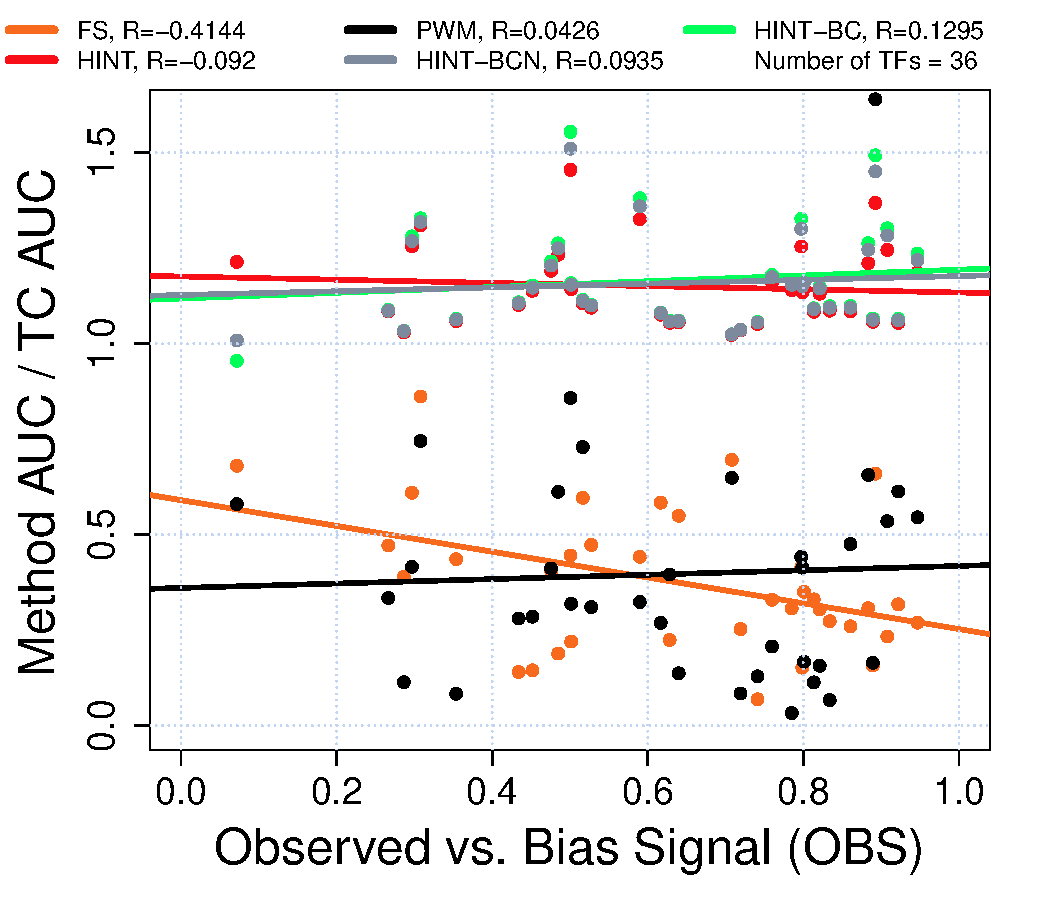
\includegraphics[width=0.70\textwidth]{Figs/BiasCorr_HeReplication.pdf}
\caption{Correlation between the performance of methods and their OBS on {\tt He Dataset}. The $x$-axis represents the observed sequence bias. The $y$-axis represents the ratio between the AUC at $10\%$ FPR for a particular method and the TC method. {\color{red!50!black}{In accordance with~\cite{he2014}, we observe that FS method has a high negative correlation (R = $-0.4144$; adjusted $p$-value $<0.001$) with the cleavage bias score, while no significant correlation is found for all other evaluated methods HINT, HINT-BCN, HINT-BC and PWM. It is important to notice that the correlation value for FS method differs from~\cite{he2014}. This stems from a different strategy to find the DNase hypersensitivity regions and MPBSs used in the evaluation dataset. Nevertheless, we were able to observe a strong bias for the FS method as in~\cite{he2014}.}}}
\label{fig:tcbiasuwk}
\end{figure}

\clearpage

\begin{figure}[t!]
\centering
\centerline{
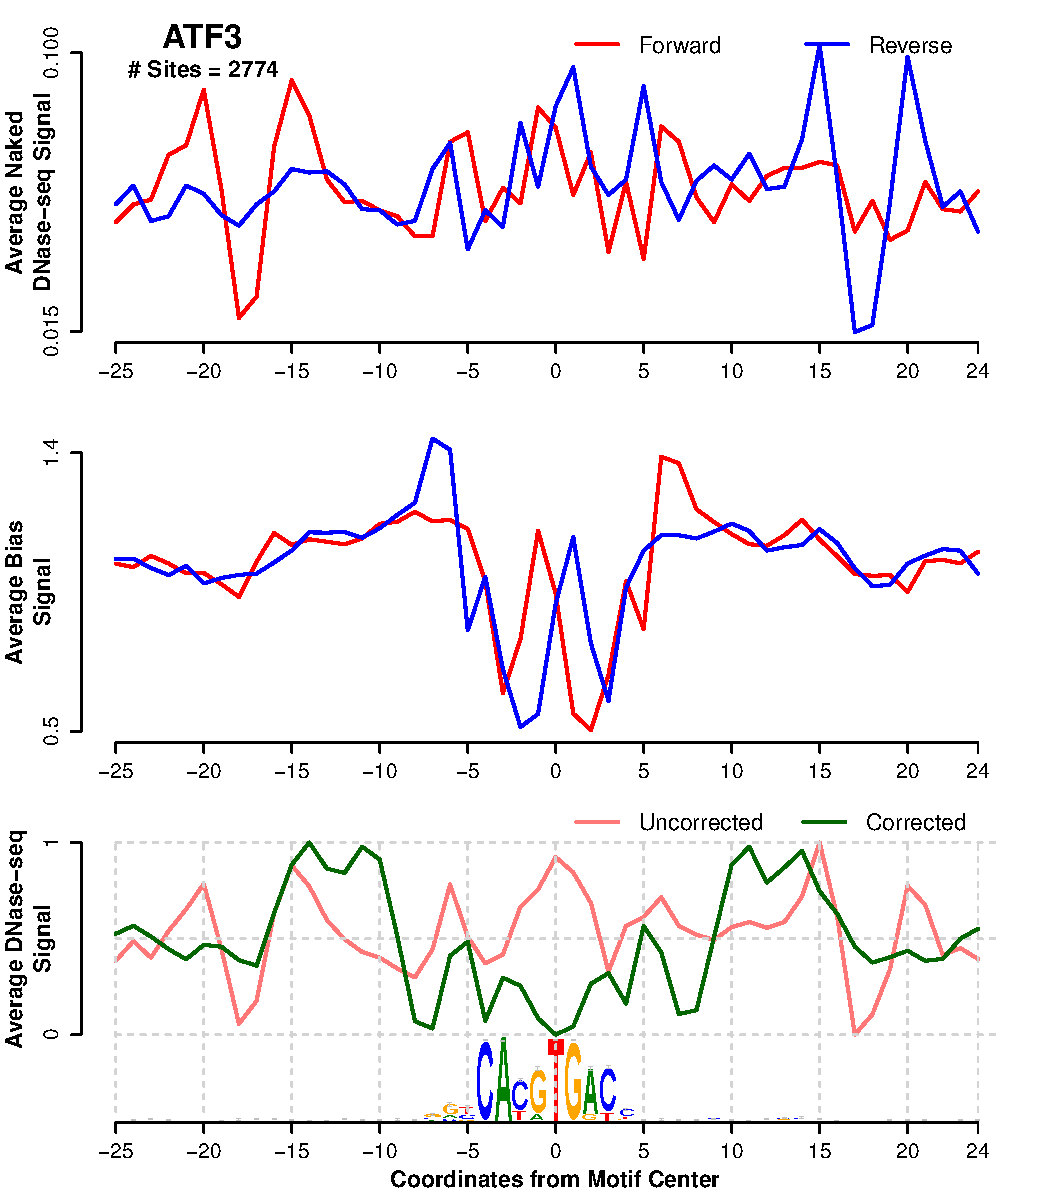
\includegraphics[width=0.33\textwidth]{Figs/BC_ATF3_PWM_H1hESC.pdf}
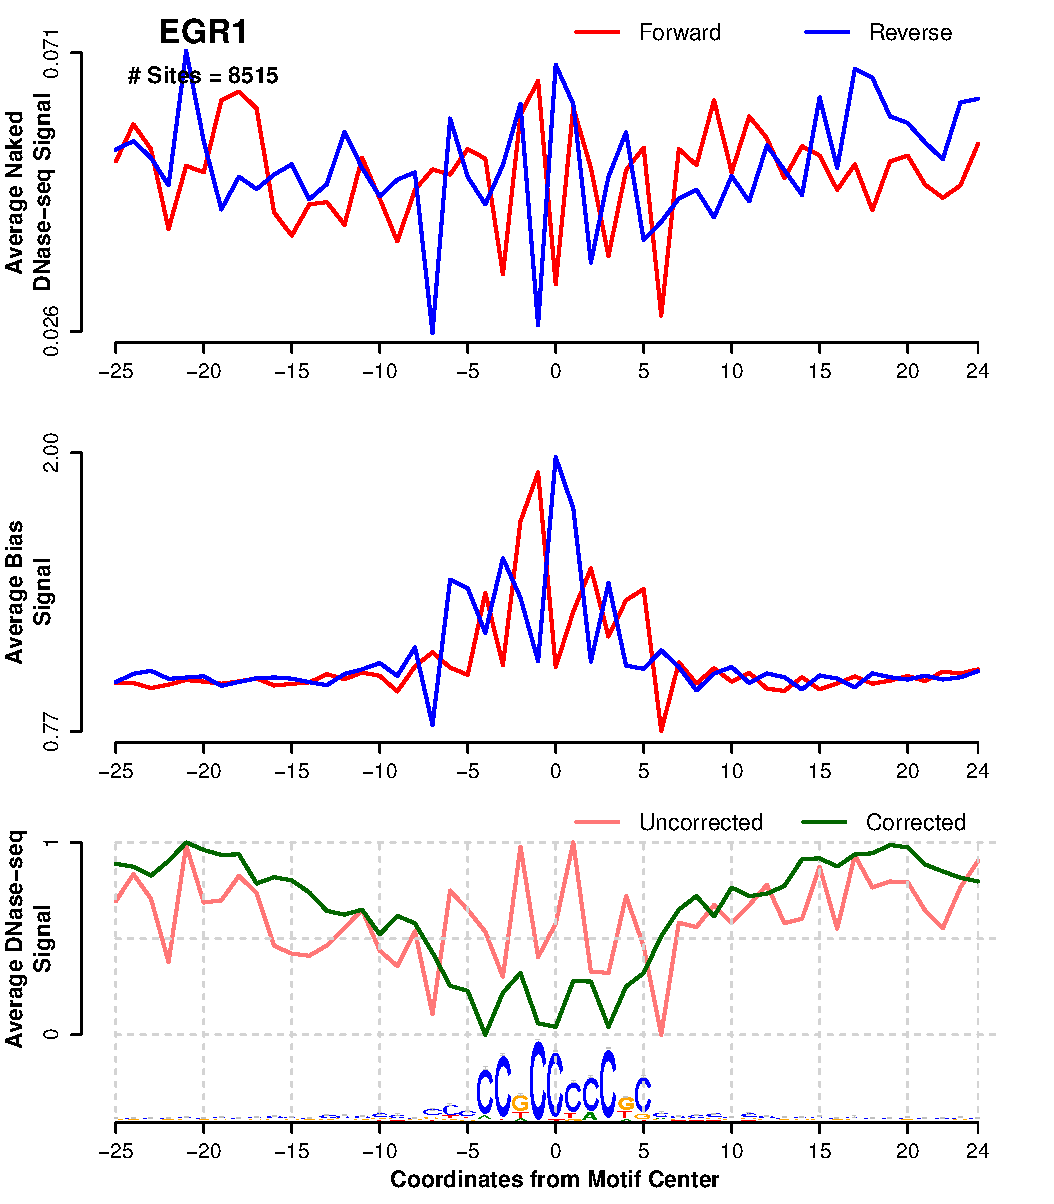
\includegraphics[width=0.33\textwidth]{Figs/BC_EGR1_PWM_H1hESC.pdf}
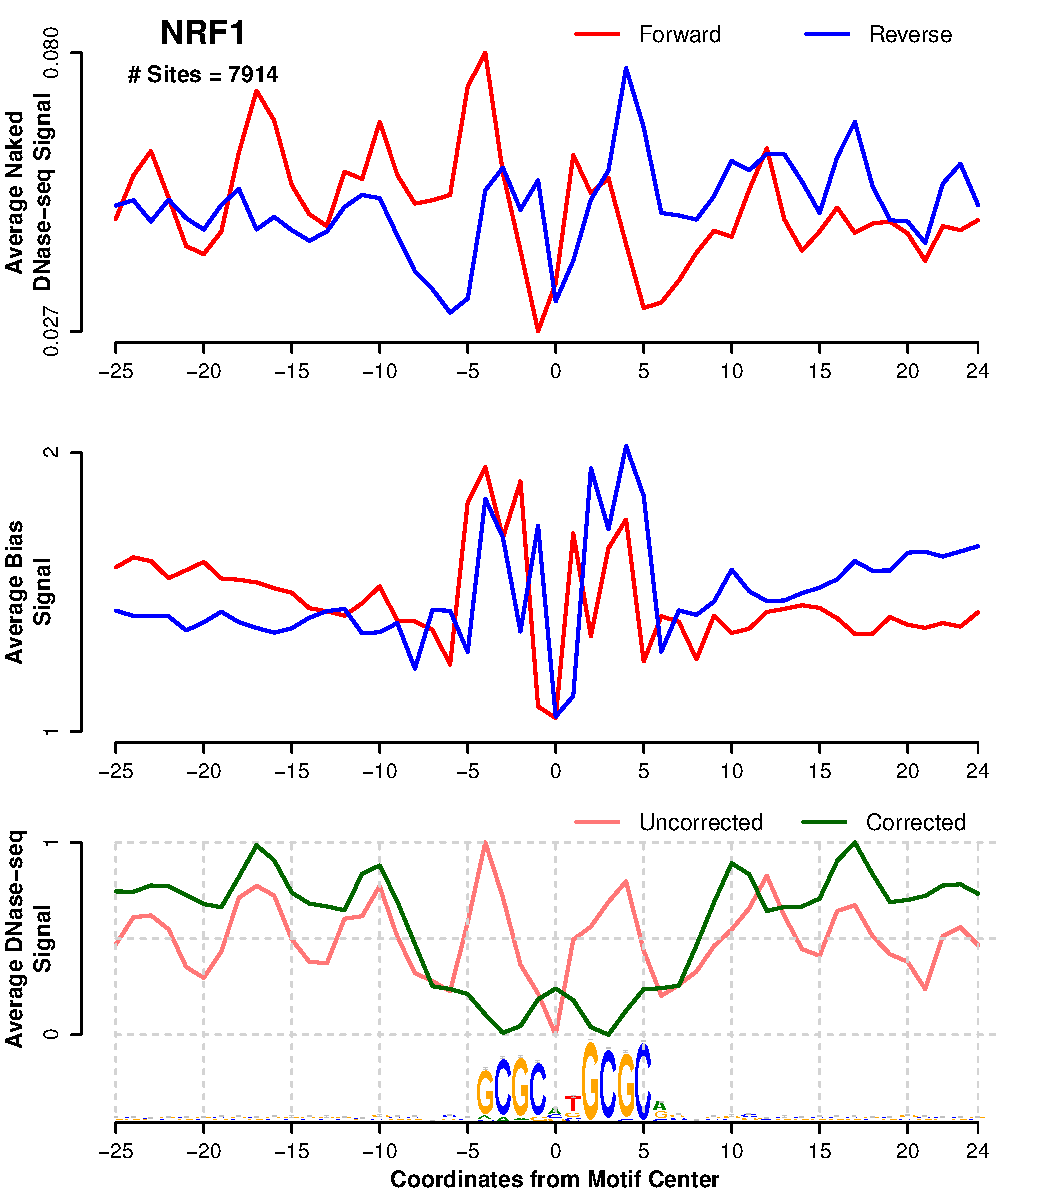
\includegraphics[width=0.33\textwidth]{Figs/BC_NRF1_PWM_H1hESC.pdf} }
\vspace{1.0cm}
\centerline{
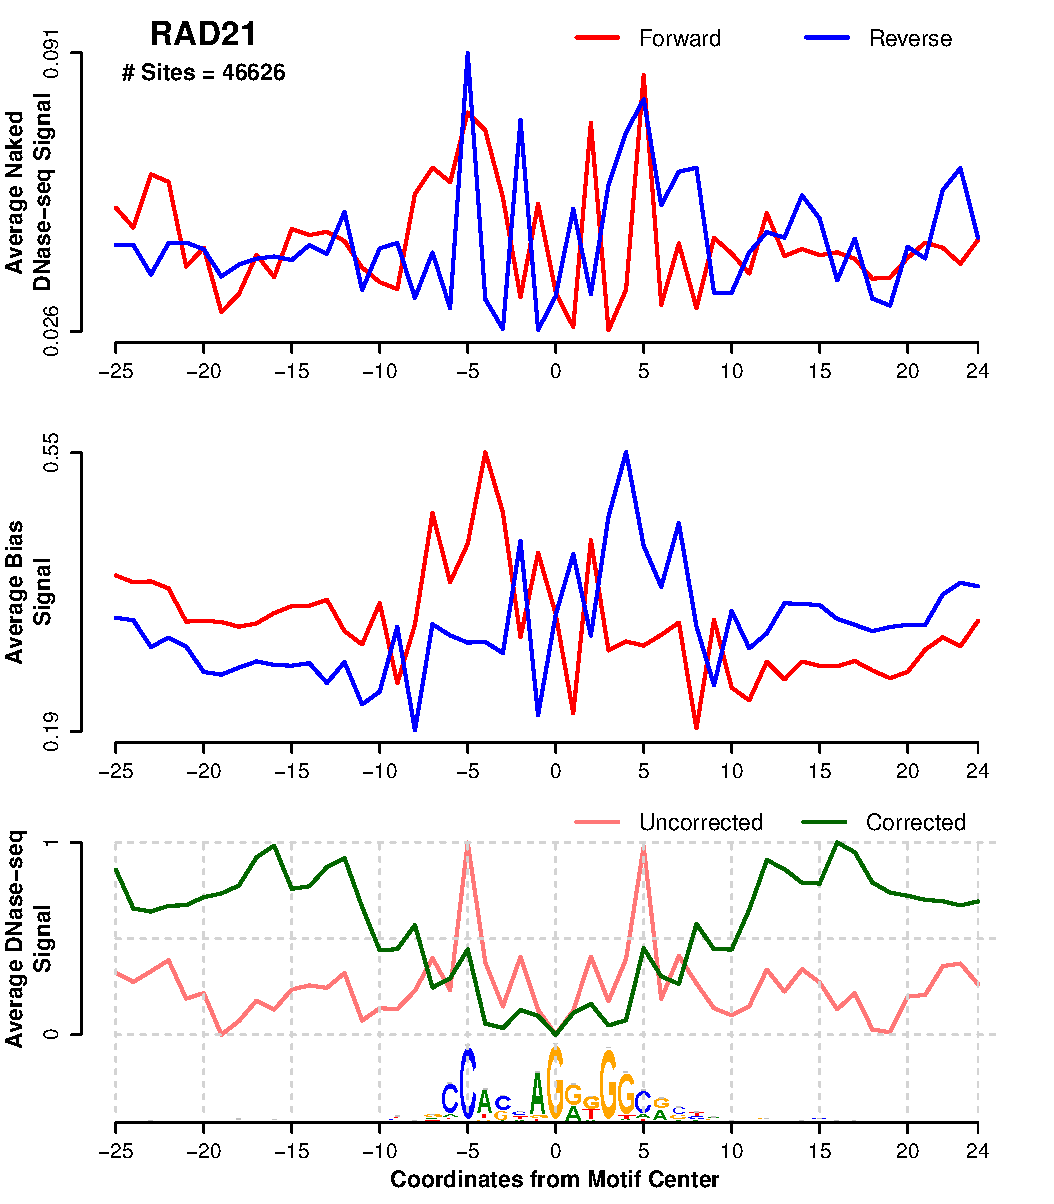
\includegraphics[width=0.33\textwidth]{Figs/BC_RAD21_PWM_H1hESC.pdf}
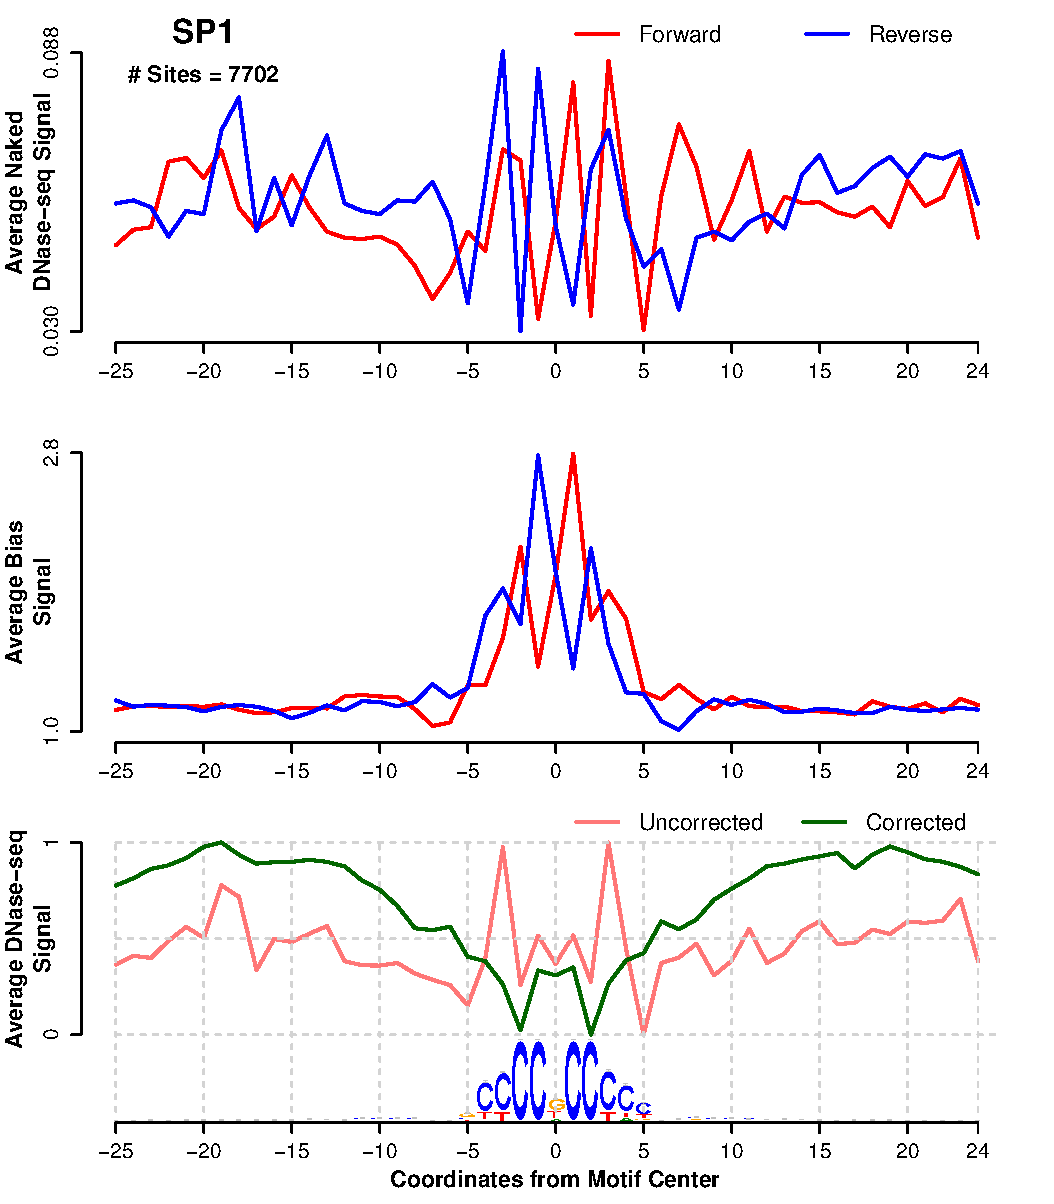
\includegraphics[width=0.33\textwidth]{Figs/BC_SP1_PWM_H1hESC.pdf}
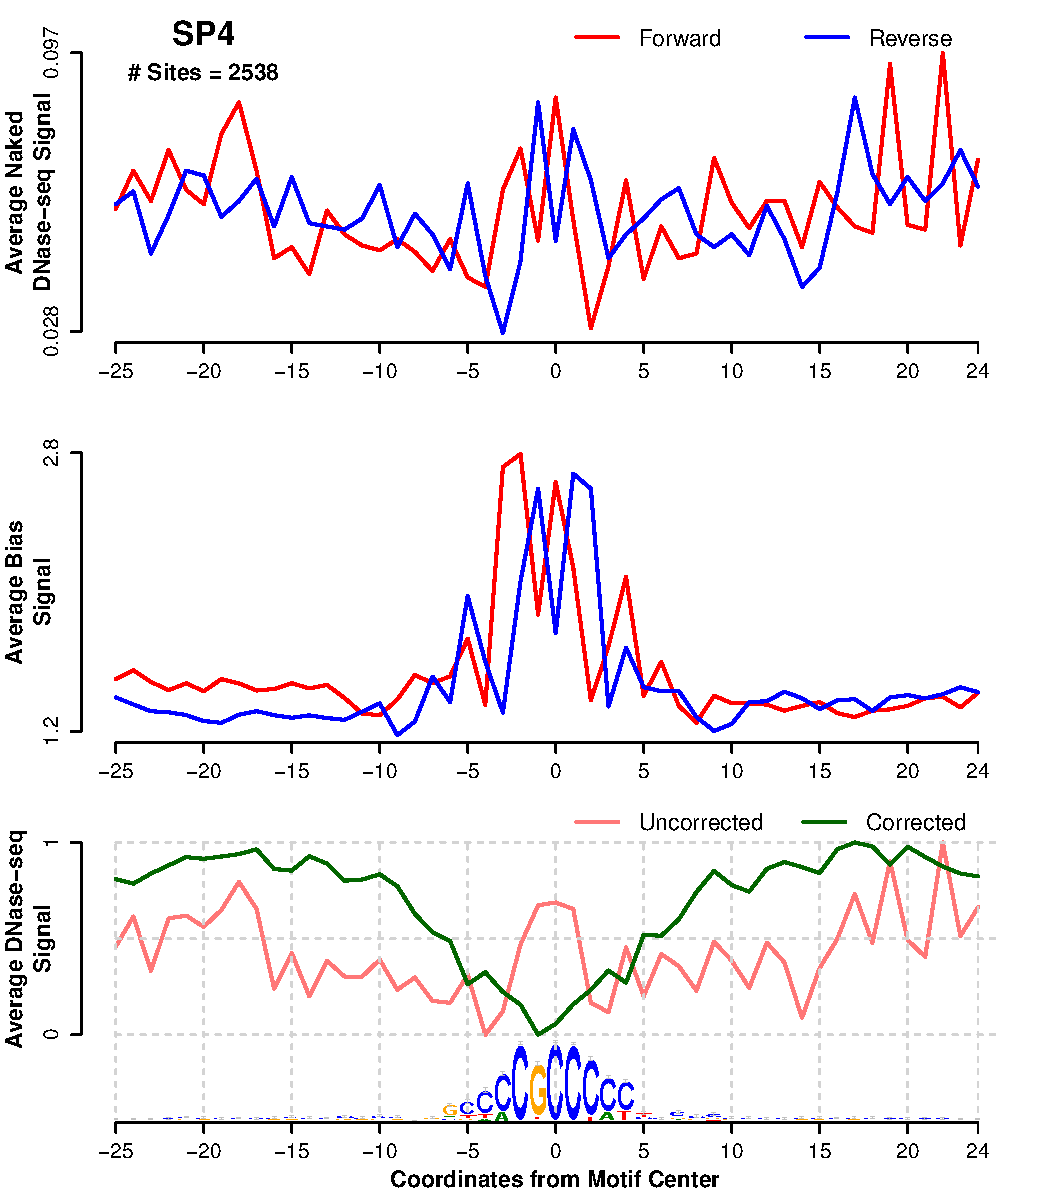
\includegraphics[width=0.33\textwidth]{Figs/BC_SP4_PWM_H1hESC.pdf}
}
\vspace{-0.1cm}
\caption{Average DNase-seq signals around selected TFs with ChIP-seq evidence in H1-hESC (DU) cell type. These TFs had the higher AUC gain between HINT-BC and HINT. {\color{red!50!black}{In the top panel, we show the strand-specific average DNase-seq signal on deproteinized DNA experiments (MCF-7 cell type); the middle panel shows the strand-specific estimated cleavage bias signal; and the bottom panels shows the (1) uncorrected -- observed DNase-seq I cleavage signal and (2) corrected -- DNase-seq signal after the bias correction by using Eq.~\ref{eq:biascorrsignal}.}} Bottom panel signals were standardized to be in [0,1]. Below the graphs, it is shown the motif logo estimated on the DNA sequences of these regions. The bias correction led to a substantial change in the average DNase I cleavage patterns surrounding several TFs. On EGR1, for instance, we observed that the bias-corrected DNase-seq signal presents three clear depletions, which fit the high affinity regions of EGR1 motif (two {\tt CC} and one {\tt C}). In contrast, EGR1 uncorrected DNase-seq signal presents a single peak in the center of the motif. The same observations can be made for other TFs, such as NRF1 (with affinity regions {\tt (C/G)(C/G)(G/C)C} and {\tt G(G/C)(C/G)(C/G)C}) and SP4 (with affinity region {\tt CGCCC}). Such patterns reflect bias corrections which are clearly beneficial to footprinting method accuracy.}
\label{fig:lineOBCsignal}
\end{figure}

\clearpage

\begin{figure}[h]
\centering
  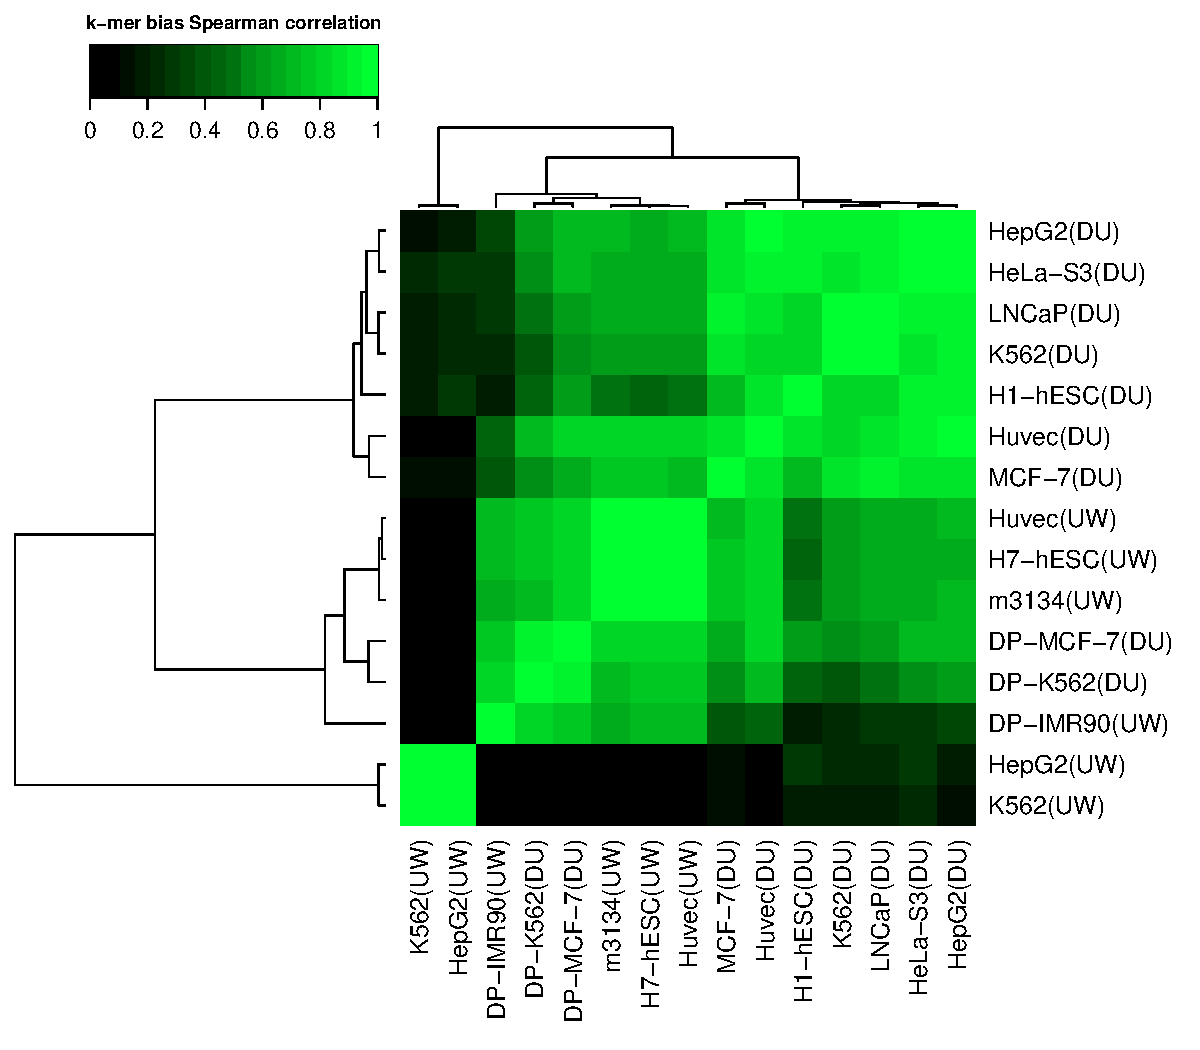
\includegraphics[width=0.7\textwidth]{Figs/Kmer_correlation_spearman.pdf}
\caption{{\color{red!50!black}{Ward's minimum variance clustering on pairwise Spearman correlation coefficient ($R$) between different DNase-seq data sets calculated based on each 6-mer $w$ ratio between observed and expected cleavage bias ($o^s_w \cdot R / r^s_w \cdot O^s$). Crawford's lab data sets are represented by ``DU'' (Duke University; single-hit protocol) and Stamatoyannopoulous' lab data sets are represented by ``UW'' (University of Washington; double-hit protocol). We observe 3 major clusters: group 1 contains all DU data sets, group 2 contains m3134, Huvec from UW and all deproteinized DNase-seq experiments (IMR90(UW); K562 and MCF-7(DU)) and group 3 contains K563 and HepG2 from UW. Correlation between experiments clustered into the same group are significant (adjusted $p$-value $<0.001$). These results confirm that DHS-estimated cleavage bias experiments from the same lab/protocol have similar bias. The only exceptions are K562(UW) and Hepg2(UW), which presented low correlation values with any other UW and DU experiments. Deproteinized DNA experiments from distinct protocols clustered together. The high correlations between deproteinized DNA experiments ($R=0.94$ for K562 and MCF-7; $R=0.81$ for K562 and IMR90) are in agreement with previous reports~\cite{yardimci2014}. In particular, deproteinized DNA experiments have a moderate correlation with experiments using the same protocols: K562 has an average $R=0.42$ with other DU experiments, MCF-7 has average $R=0.60$ with other DU experiments; while IMR90 has average $R=0.67$ with m3134(UW) and Huvec(UW). While deproteinized DNA could be used for estimation bias correction for experiments with same protocol, we observe a lack of correlation between deproteinized IMR90(UW) and K562/HepG2(UW) experiments. One possible reason is that small variations of the same protocol might introduce further cleavage bias. }}}
\label{fig:datasetcorr}
\end{figure}

\clearpage

\begin{figure}[h!]
\centering
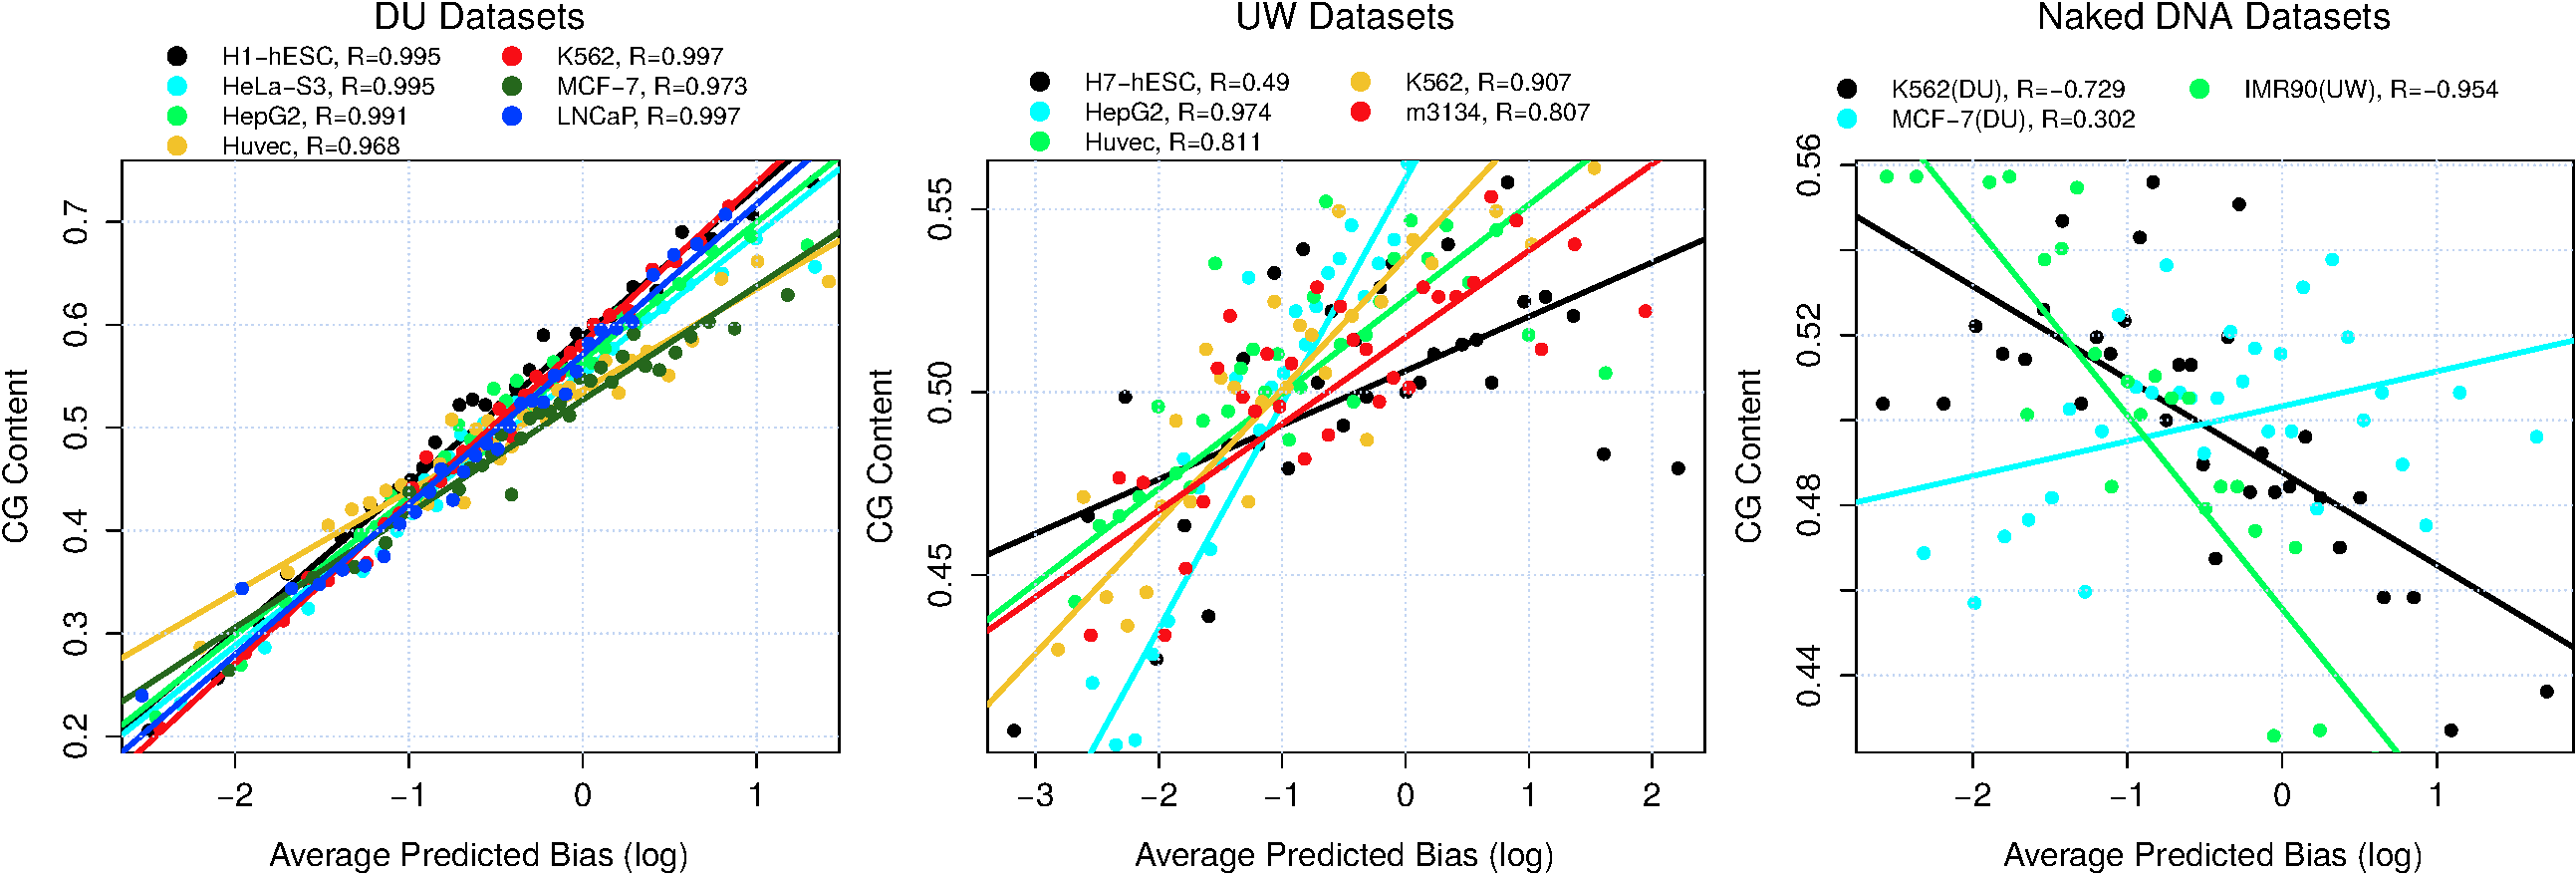
\includegraphics[width=1.0\textwidth]{Figs/CgBiasCorr.pdf}
\caption{{\color{red!50!black}{Association between k-mer CG content and cleavage bias. We sorted k-mers by their cleavage bias estimate and grouped similar ranked k-mers in 32 groups.
%The number of groups was chosen as a balance between statistical significance ($>$ 30 data points) and CG estimation significance ($>$ 100 k-mers per group).
We show scatter plots with CG content vs. average cleavage bias for k-mer groups on DHS-based k-mers estimated from single-hit (DU), double-hit (WU) and naked DNA experiments. There is a strong positive correlation between cleavage bias and CG content for all DHS-based estimates from both single-hit and double-hit protocols (adjusted p-value < 0.01). Interestingly, we observe a negative correlation for two deproteinized DNA experiments: K562(DU) and IMR90(UW) (adjusted p-value < 0.00001). These results reinforce the distinctions between naked DNA and DHS-based cleavage bias estimates. Moreover, it explains the positive impact of cleavage bias correction on TFs with CG-rich motifs, as the ones described in Supplementary Figure~\ref{fig:lineOBCsignal}.
}}}
\label{fig:bias_cg}
\end{figure}

% XXX - EG - improve figure

\clearpage

\begin{figure}[h!]
\centering
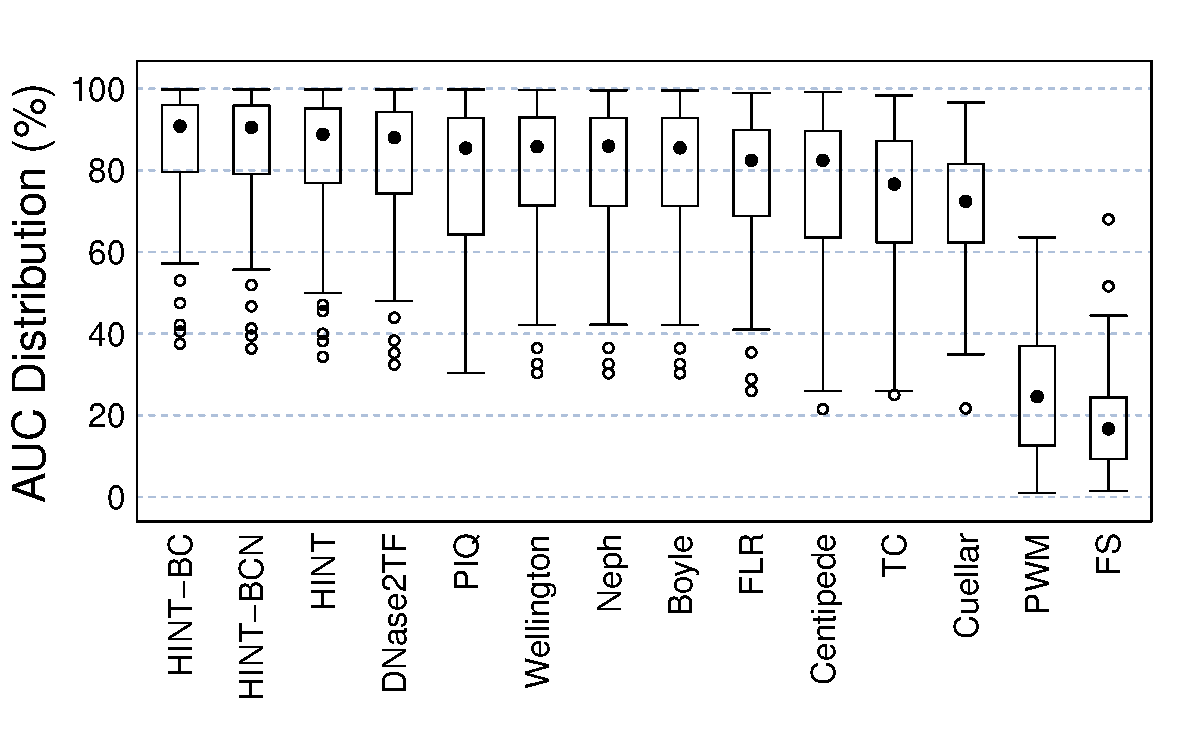
\includegraphics[width=0.8\textwidth]{Figs/AUC_Boxplot.pdf}
\caption{{\color{red!50!black}{AUC distribution for 14 footprinting methods regarding all validation sets (ordered by median AUC). We used the Friedman-Nemenyi ranking and hypothesis test for statistical evaluation~\citep{demsar2006} (Supplementary Tables~\ref{tab:fn.table}). All segmentation-based approaches (HINT-BC, HINT-BCN, HINT, Boyle, DNase2TF and Wellington) and the site centric method PIQ significantly outperformed TC (adjusted $p$-value $< 0.01$). Moreover, HINT-BC and HINT-BCN outperformed all other competing methods (adjusted $p$-value $< 0.01$). As reported in~\cite{he2014}, the AUC of the TC approach was significantly higher than FS method (adjusted $p$-value $< 0.01$).}}}
\label{fig:auc_boxplot}
\end{figure}

\clearpage

\begin{figure}[t!]
\centering
\centerline{
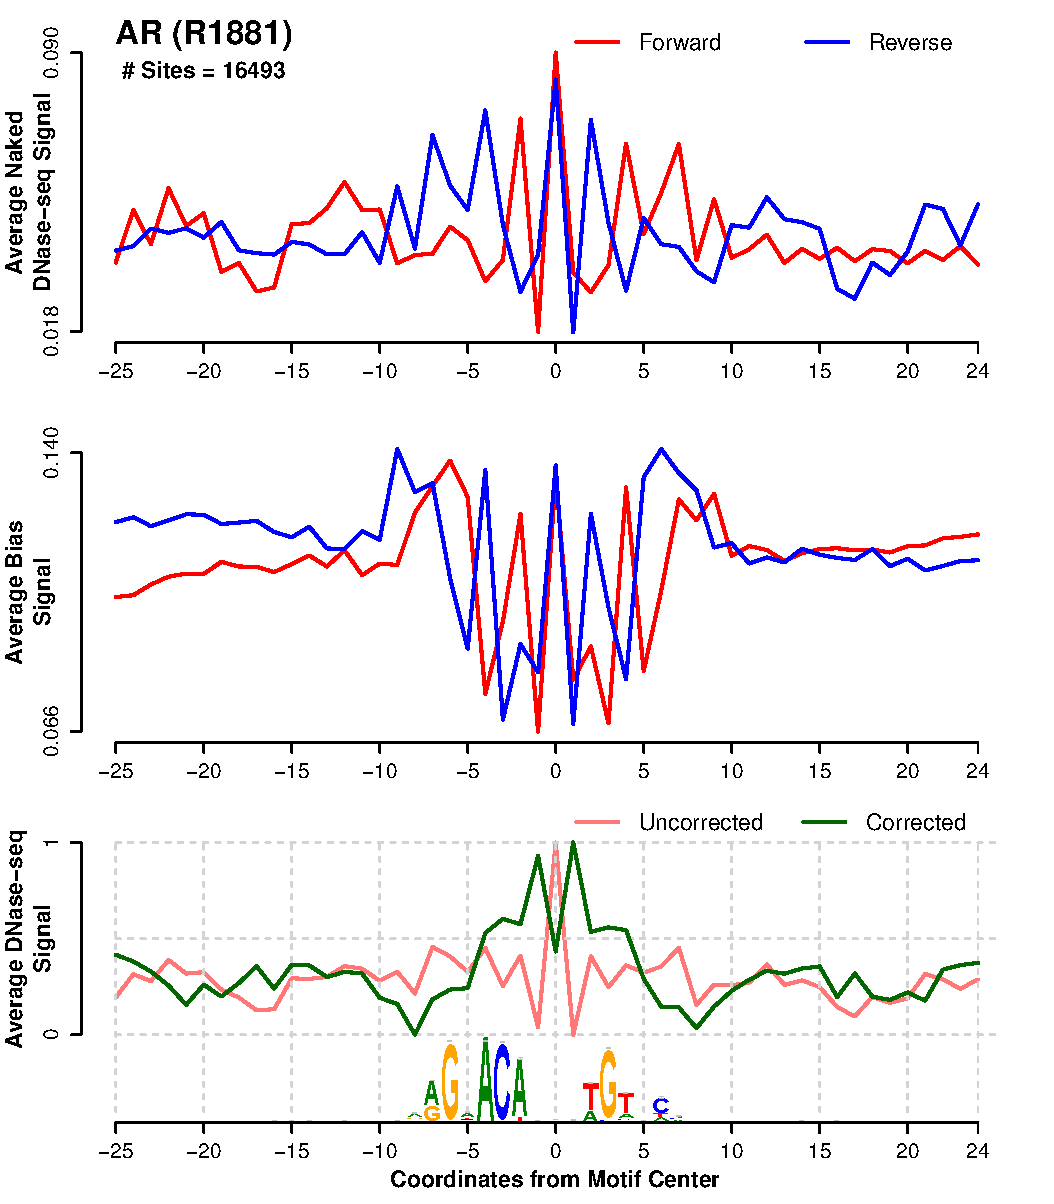
\includegraphics[width=0.38\textwidth]{Figs/BC_AR_R1881_PWM_LnCaP.pdf}
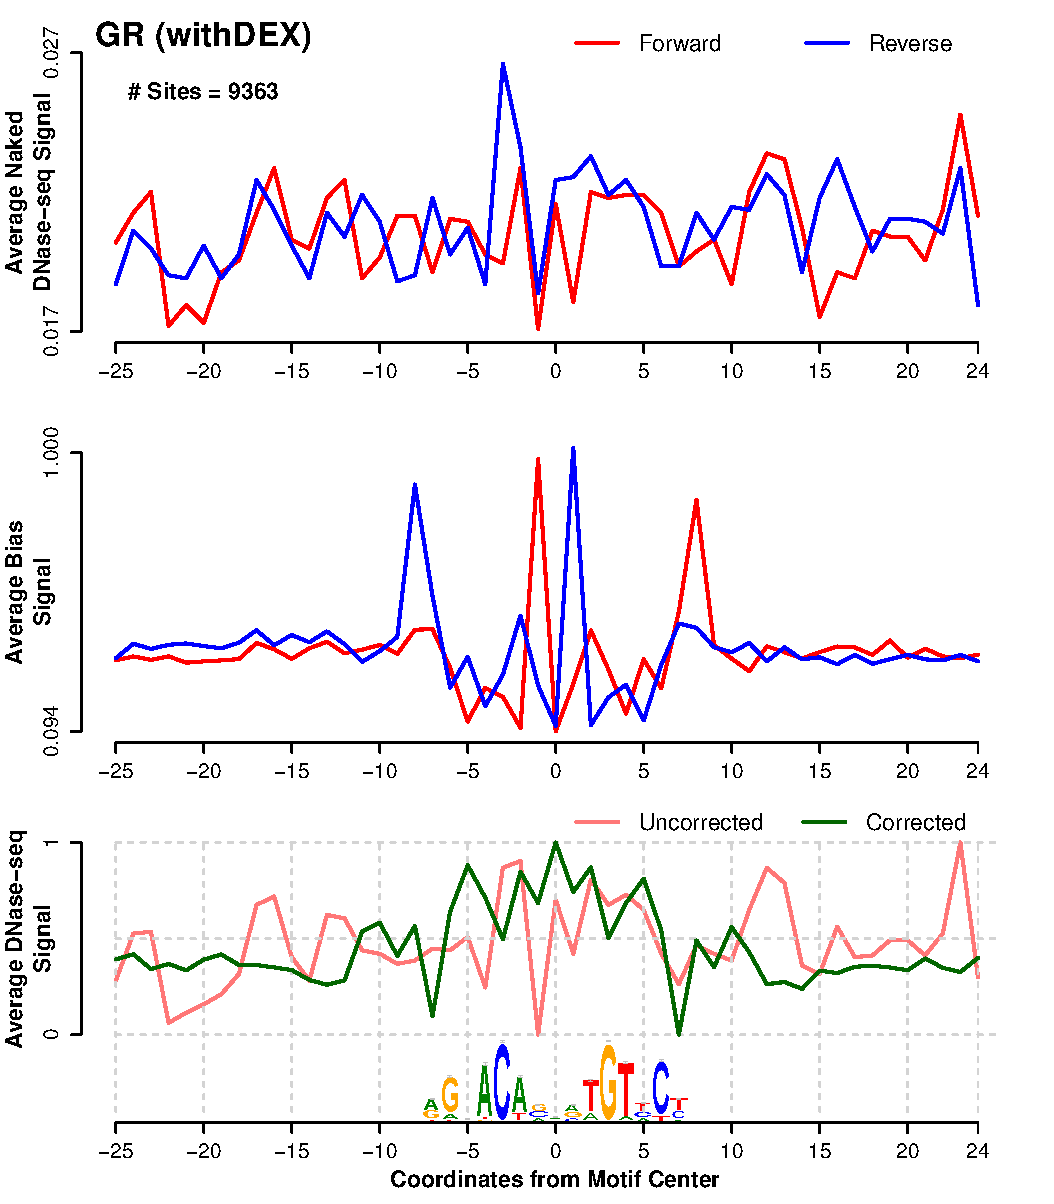
\includegraphics[width=0.38\textwidth]{Figs/BC_GR_withDEX_PWM_m3134.pdf} }
\vspace{0.4cm}
\centerline{
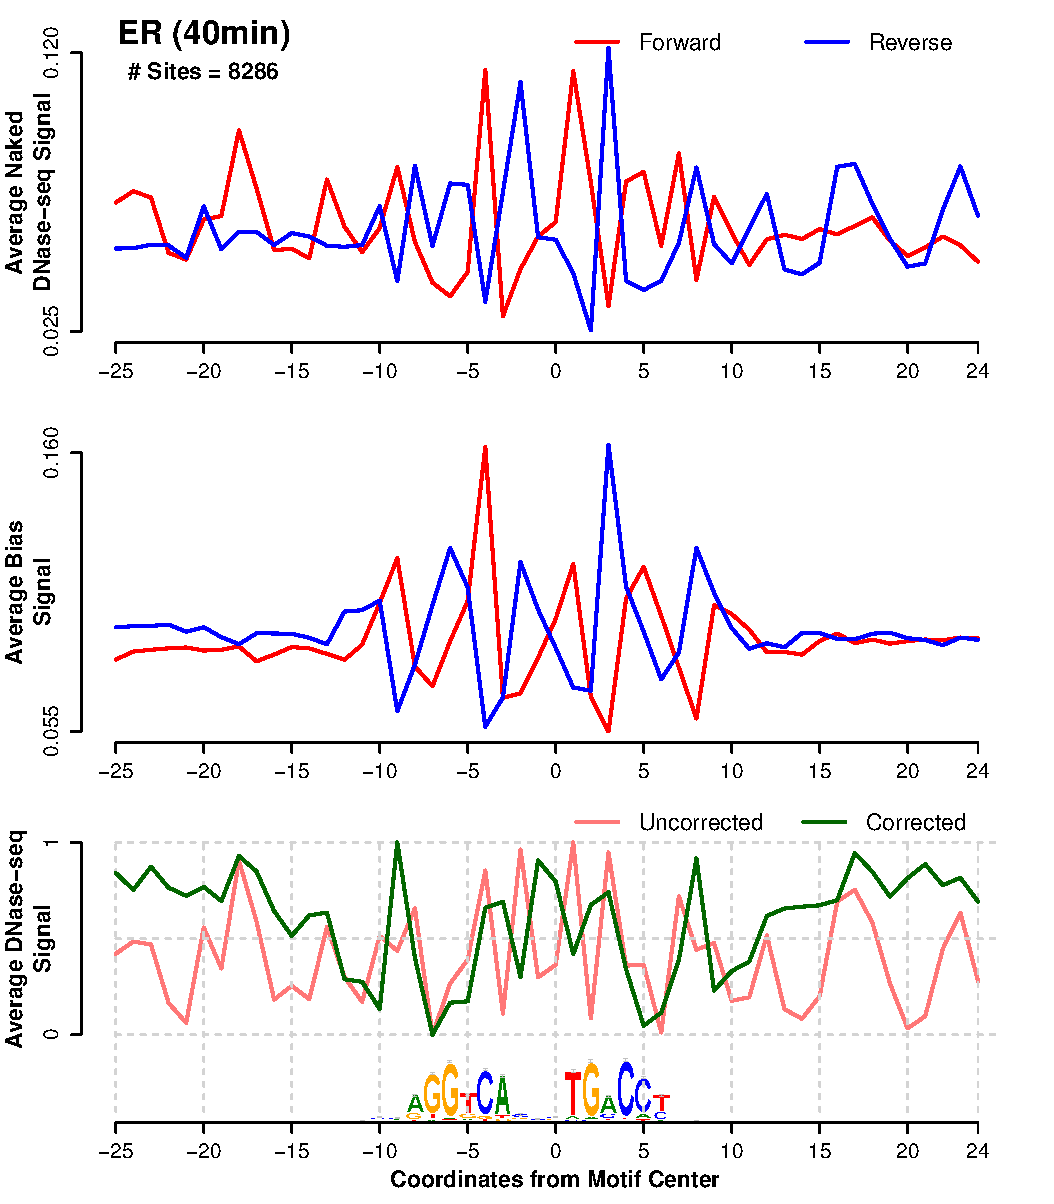
\includegraphics[width=0.38\textwidth]{Figs/BC_ER_40min_PWM_Mcf7.pdf} 
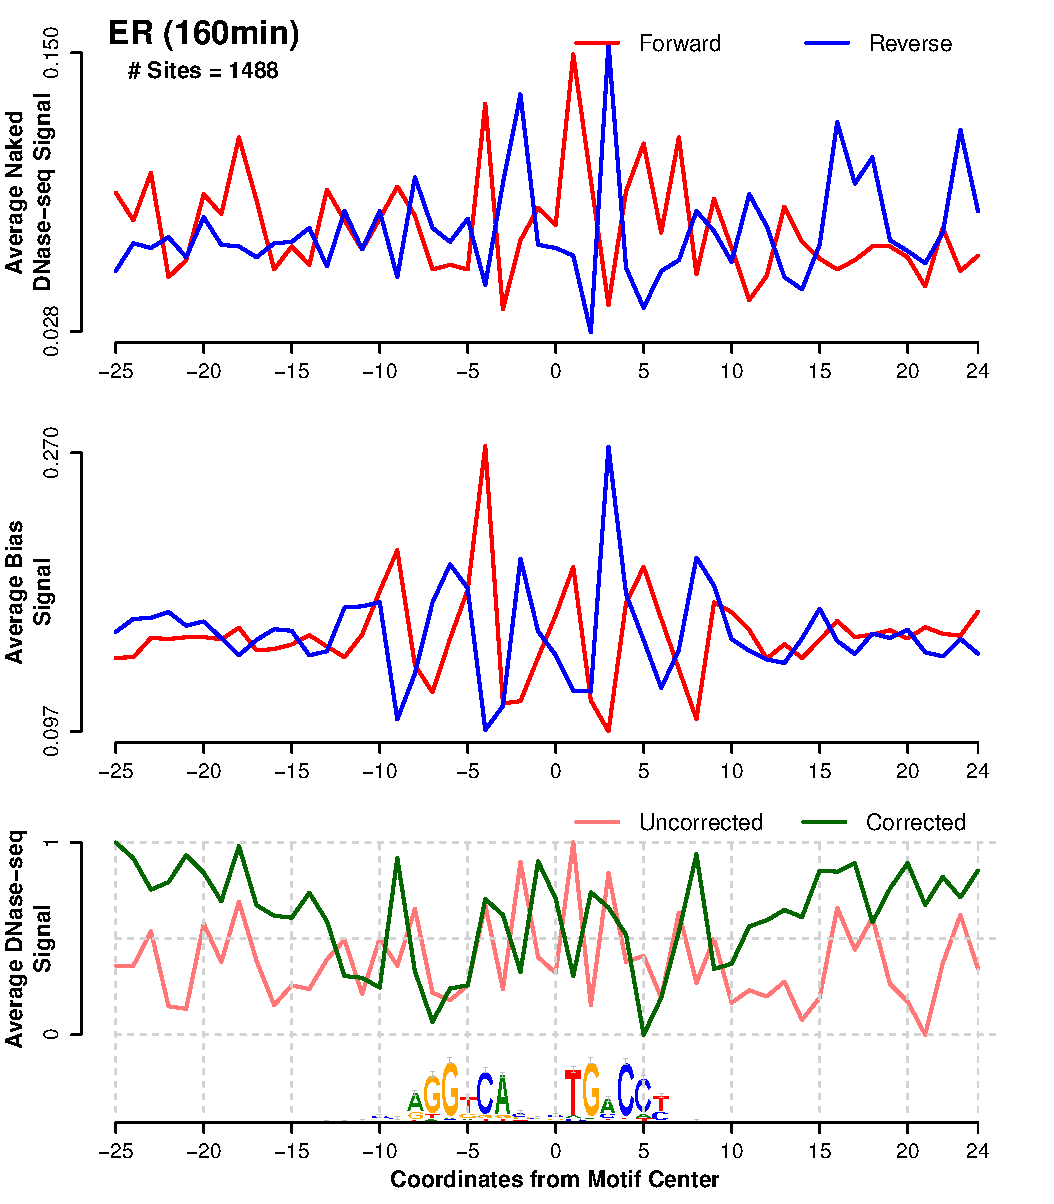
\includegraphics[width=0.38\textwidth]{Figs/BC_ER_160min_PWM_Mcf7.pdf} }
\vspace{-0.1cm}
\caption{{\color{red!50!black}{Average DNase-seq signals around nuclear receptor TFs with ChIP-seq evidence in LNCaP(DU), m3134(UW) and MCF-7(DU) cell types. In the top panel, we show the strand-specific average DNase-seq signal on deproteinized DNA experiments (MCF-7(DU) for data sets from single hit and IMR90(UW) for data sets with double-hit protocol); the middle panel shows the strand-specific estimated cleavage bias signal; and the bottom panels shows the (1) uncorrected -- observed DNase-seq I cleavage signal and (2) corrected -- DNase-seq signal after the bias correction by using Eq.~\ref{eq:biascorrsignal}. Bottom panel signals were standardized to be in [0,1]. Below the graphs, it is shown the motif logo estimated on the DNA sequences of these regions. While corrected DNase-seq profiles from ER have a better match with the underlying motif, this is not the case for AR and GR. However, we observed a small gain in the AUC score comparing HINT-BC and HINT. This difference is in the upper quartile range for all 233 TFs analyzed. These results indicate that cleavage bias correction also brings improvements to footprint prediction of nuclear receptors. However, all these factors have low AUC scores in all footprinting methods, i.e. lower quartiles for HINT-BC or TC AUC score. This indicates that short binding time indeed poses a challenge in footprint prediction.}}}
\label{fig:lineOBCsignal2}
\end{figure}

\clearpage

\begin{figure}[h!]
\centering
\centerline{
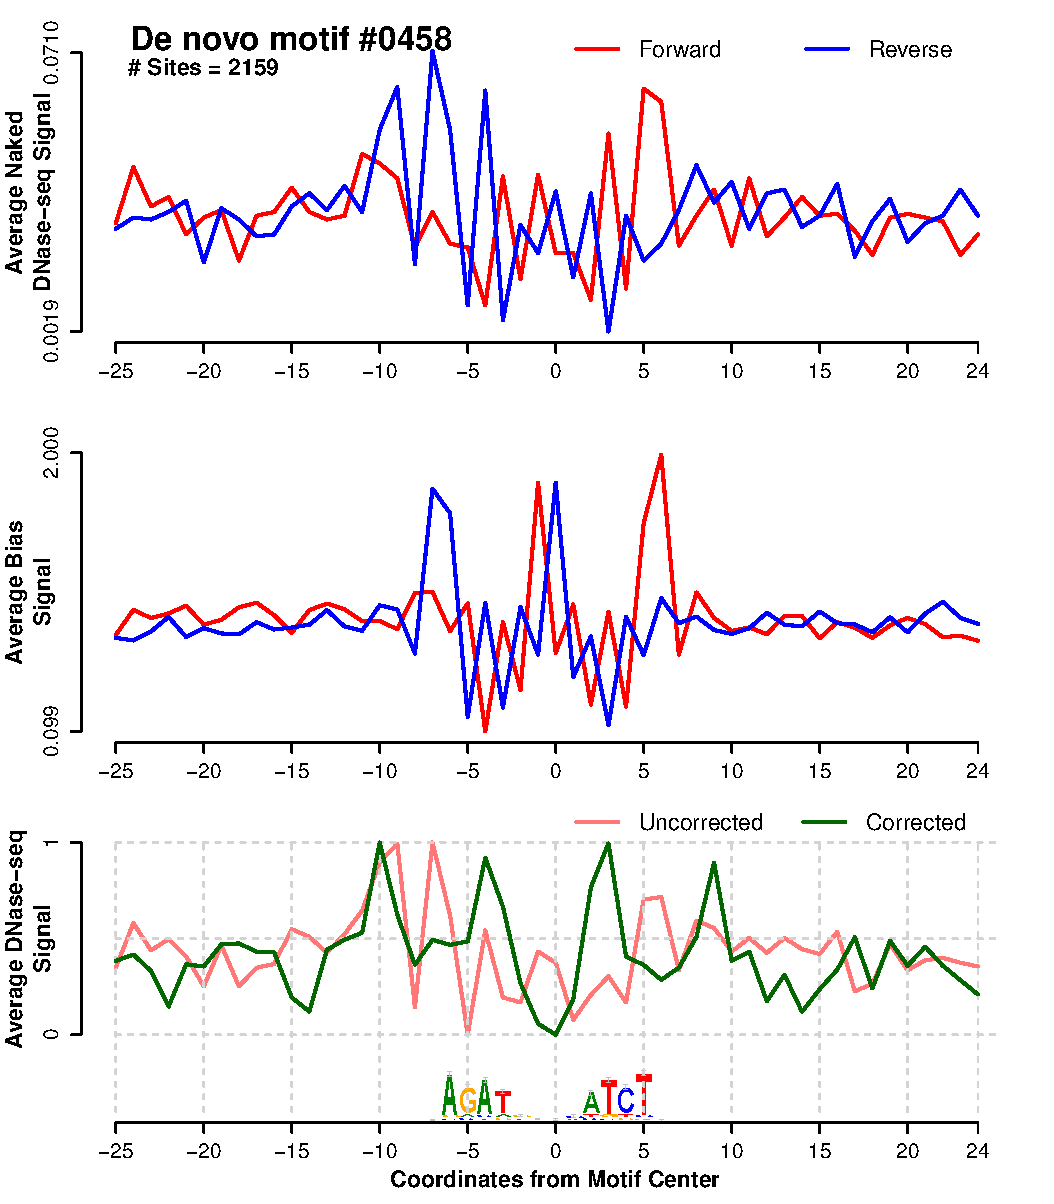
\includegraphics[width=0.5\textwidth]{Figs/BC_0458_PWM_H7hesc.pdf}
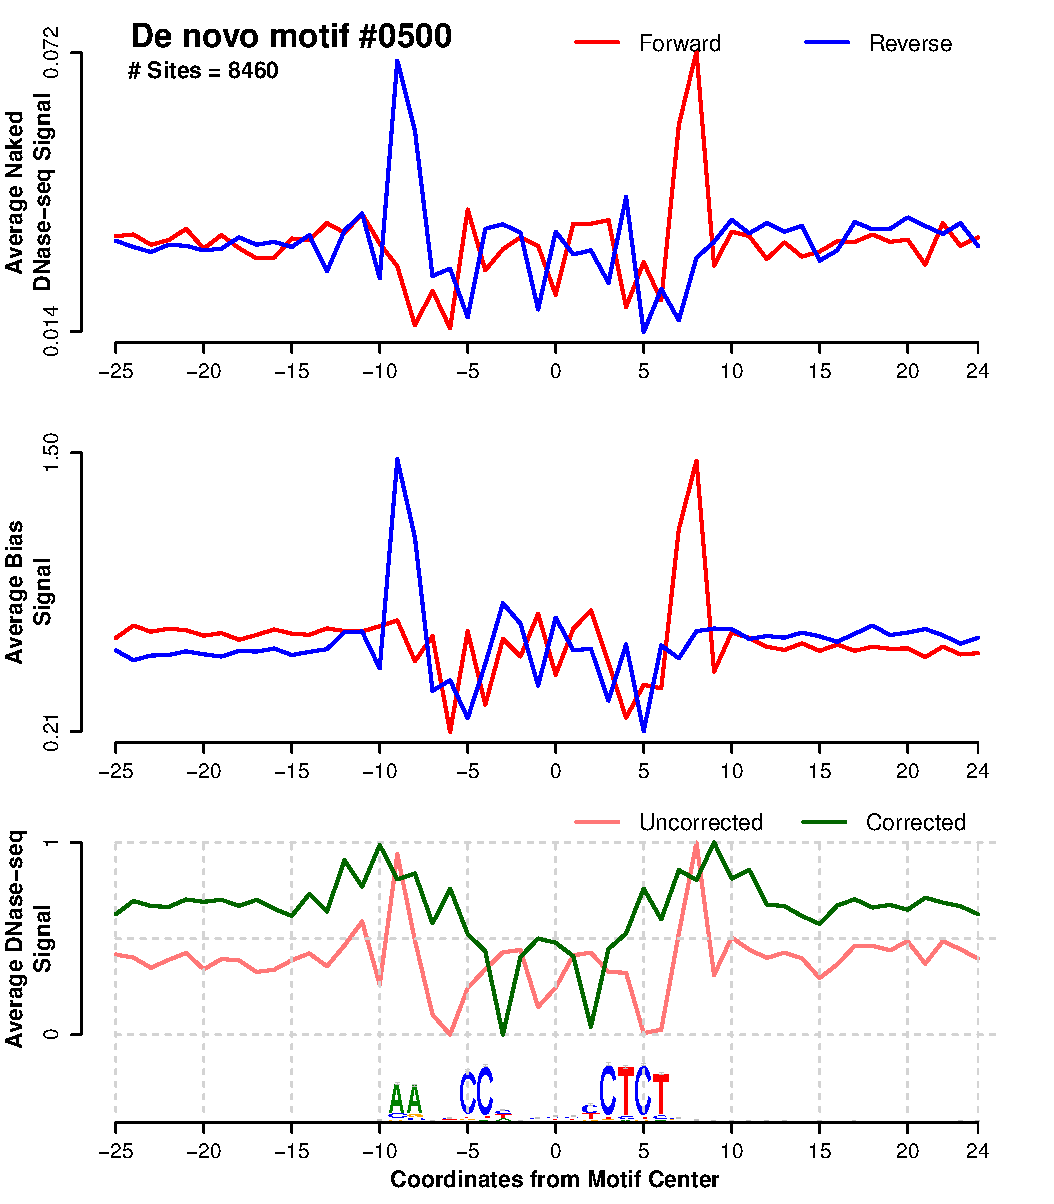
\includegraphics[width=0.5\textwidth]{Figs/BC_0500_PWM_H7hesc.pdf}
}
\vspace{-0.1cm}
\caption{{\color{red!50!black}{Average bias and DNase-seq signals around binding sites of \emph{de novo} motifs 0458 and 0500 on cell type H7-hESC. In the top panel, we show the strand-specific average DNase-seq signal on deproteinized DNA experiments (MCF-7 cell type); the middle panel shows the strand-specific estimated cleavage bias signal; and the bottom panels shows the (1) uncorrected -- observed DNase-seq I cleavage signal and (2) corrected -- DNase-seq signal after the bias correction by using Eq.~\ref{eq:biascorrsignal}. Bottom panel signals were standardized to be in [0,1]. Below the graphs, it is shown the motif logo estimated on the DNA sequences of these regions. These motifs were discovered in the footprint analysis of~\cite{neph2012a} and indicated in~\cite{he2014} to be artifacts of cleavage bias. Cleavage bias-corrected DNase-seq profiles reveal no clear footprint shape. Furthermore, we compared the overlap between footprints generated by HINT-BC and Neph in H7-hESC(UW) cells. We considered only the MPBSs that overlapped DHSs in H7-hESC. We observed that 24.99\% (motif 0458) and 28.58\% (motif 0500) of MPBSs associated with a Neph footprint. In contrast, only 0.73\% (motif 0458) and 1.71\% (motif 0500) of MPBSs overlapped with a HINT-BC footprint. Altogether, this indicates that these motifs are indeed potential artifacts of cleavage bias and reinforces the importance of bias correction prior to any DNase-seq analysis.}}}
\label{fig:denovo}
\end{figure}

\clearpage

%%%%%%%%%%%%%%%%%%%%%%%%%%%%%%%%%%%%%%%%%%%%%%%%%%%%%%%%%%%%%%%%%%%%%%%%%%%%%%%
% Tables
%%%%%%%%%%%%%%%%%%%%%%%%%%%%%%%%%%%%%%%%%%%%%%%%%%%%%%%%%%%%%%%%%%%%%%%%%%%%%%%

\setcounter{table}{0}

\begin{table}[h]
\begin{center}
\caption{Summary of DNase-seq data.}
\label{tab:dataencode}
\renewcommand{\arraystretch}{1.2}
\begin{tabularx}{\textwidth}{ lllXr }
\hline
Cell Type & Lab                 & UCSC             & GEO/NCBI                     & \# Mapped Reads \\
\hline
H1-hESC   & Crawford            & wgEncodeEH000556 & GSM816632                    & 110303078       \\
HeLa-S3   & Crawford            & wgEncodeEH000540 & GSM816643                    & 54267867        \\
HepG2     & Crawford            & wgEncodeEH000537 & GSM816662                    & 50838536        \\
Huvec     & Crawford            & wgEncodeEH000548 & GSM816646                    & 31848532        \\
K562      & Crawford            & wgEncodeEH000530 & --                           & 365820647       \\
LNCaP     & Crawford            & wgEncodeEH001097 & GSM816637                    & 163625945       \\
MCF-7     & Crawford            & wgEncodeEH000579 & GSM816627                    & 89113893        \\
K562*     & Crawford            & --               & GSM1496625                   & 202001412       \\
MCF-7*    & Crawford            & --               & GSM1496626                   & 210715393       \\
H7-hESC   & Stamatoyannopoulous & wgEncodeEH000511 & GSM736638 \newline GSM736610 & 302050785       \\
HepG2     & Stamatoyannopoulous & wgEncodeEH000482 & GSM736637 \newline GSM736639 & 168883956       \\
Huvec     & Stamatoyannopoulous & wgEncodeEH000488 & GSM736575 \newline GSM736533 & 429088276       \\
K562      & Stamatoyannopoulous & wgEncodeEH000484 & GSM736629 \newline GSM736566 & 179970820       \\
m3134     & Stamatoyannopoulous & wgEncodeEM001721 & GSM1014196                   & 127594903       \\
IMR90*    & Stamatoyannopoulous & --               & SRA068503                    & 138604440       \\
\hline
\multicolumn{5}{l}{*Deproteinized DNase-seq experiments.} \\
\end{tabularx}
\end{center}
\end{table}

\clearpage

\begin{table}[h]
\begin{center}
\caption{{\color{red!50!black}{Summary of computational footprinting methods. We characterize distinct methods based on: (1) the approach used for detection of footprints (site-centric or segmentation-based); (2) presence of a smoothing technique on DNase-seq signals; (3) correction of cleavage bias; (4) bias-correction strategy; (5) whether the method is affected by cleavage bias and (6) whether the method significantly outperforms TC. Concerning bias invariance, methods that perform bias-correction of 6-mers (FLR, HINT-BC, HINT-BCN) or that work on smoothed signals (PIQ and Cuellar) do not have their performance influenced by cleavage bias. Note that the DNase2TF implementation only allows the use of 2 or 4-mers and would be possibly improved if 6-mers were supported. Moreover, smoothing of DNase-seq signal as performed by PIQ and Cuellar is also an alternative to implicitly correct for cleavage bias. Concerning prediction performance, all segmentation-based methods (with the exception of Neph) are able to outperform TC prediction performance, while the only site-centric method outperforming TC is PIQ. This indicates an advantage of segmentation-based approaches on the footprint detection problem. Moreover, segmentation-based methods are simpler to execute (single run per DNase-seq experiment) and worked well with default parameters. It is important to point that there is no code available for Boyle method, which makes its usage on further DNase-seq experiments not possible. Neph, Welligton and DNase2Tf methods are based on optimization of flanking regions to estimate FS-like scores. DNase2TF, which is only outperformed by HINT methods, is another good option. DNase2TF did not require extra parametrization and its execution was very straightforward. Site-centric approaches, as PIQ, FLR and Centipede, are estimated for each motif at hand. We have previously observed that Centipede EM-like algorithm has convergence problems for particular factors and required extra parametrization experiments~\cite{gusmao2014}. This was particularly the case for TF data sets with higher number of MPBSs and high proportion of MPBSs not supported by ChIP-seq (negative examples). A similar behavior is also observed for FLR, which also required the execution of several initializations to avoid numerical problems. Indeed, we could not obtain FLR results for 3 TFs (REST binding on H1-hESC(DU) and K562(DU) and MEF2A binding on H1-hESC(DU)) after executing jobs for 3 weeks. Concerning Cuellar method, its poor predicted performance is due to its simplistic model for the DNase-seq data; average amount of DNase-seq reads on 200 bp reads. PIQ, which has overall good performance, did not show factor-specific issues or required further parametrization experiments. Also, its implementation allows for the execution on several motifs at a time without large computational demand.}}}
\label{tab:summary}
\renewcommand{\arraystretch}{1.2}
\begin{tabularx}{\textwidth}{ cccc|XX }
\hline
Method     & Type         & Smoothing & Bias        & Invariance & Improve \\
           &              &          & Correction  & Bias       & TC      \\
\hline
Centipede  & site-centric &          &             &            &         \\
Neph       & segmentation &          &             &            &         \\
FLR        & site-centric &          & 6-mers      & X          &         \\
Cuellar    & site-centric & X        &             & X          &         \\
Wellington & segmentation &          &             &            & X       \\
Boyle      & segmentation &          &             &            & X       \\
DNase2TF   & segmentation &          & 4-mers      &            & X       \\
PIQ        & site-centric & X        &             & X          & X       \\
HINT       & segmentation &          &             & X          & X       \\
HINT-BC    & segmentation &          & 6-mers      & X          & X       \\
HINT-BCN   & segmentation &          & 6-mers      & X          & X       \\
\hline
\end{tabularx}
\end{center}
\end{table}

\clearpage

\begin{table}[h!]
\vspace{0.0cm}
\begin{center}
\caption{Friedman-Nemenyi hypothesis test results on AUC for all evaluated methods. The asterisk and the cross, respectively, indicate that the method in the column outperformed the method in the row with significance levels of 0.01 and 0.05}
\label{tab:fn.table}
\vspace{0.5cm}
\renewcommand{\arraystretch}{1.2}
  \begin{tabular}{ rcccccccccccccc }
    & \rotatebox{90}{HINT-BC} & \rotatebox{90}{HINT-BCN} & \rotatebox{90}{HINT} & \rotatebox{90}{DNase2TF} & \rotatebox{90}{PIQ} & \rotatebox{90}{Wellington} & \rotatebox{90}{Neph} & \rotatebox{90}{Boyle} & \rotatebox{90}{FLR} & \rotatebox{90}{Centipede} & \rotatebox{90}{Cuellar} & \rotatebox{90}{TC} & \rotatebox{90}{PWM} & \rotatebox{90}{FS} \\
    \hline
    HINT-BC &     &     &     &     &     &     &     &     &     &     &     &     &     &     \\
    HINT-BCN &     &     &     &     &     &     &     &     &     &     &     &     &     &     \\
    HINT & $*$ &     &     &     &     &     &     &     &     &     &     &     &     &     \\
    DNase2TF & $*$ & $+$ &     &     &     &     &     &     &     &     &     &     &     &     \\
    PIQ & $*$ & $*$ & $+$ &     &     &     &     &     &     &     &     &     &     &     \\
    Wellington & $*$ & $*$ & $*$ & $*$ &     &     &     &     &     &     &     &     &     &     \\
    Neph & $*$ & $*$ & $*$ & $*$ &     &     &     &     &     &     &     &     &     &     \\
    Boyle & $*$ & $*$ & $*$ & $*$ &     &     &     &     &     &     &     &     &     &     \\
    FLR & $*$ & $*$ & $*$ & $*$ & $*$ & $*$ & $*$ &     &     &     &     &     &     &     \\
    Centipede & $*$ & $*$ & $*$ & $*$ & $*$ & $*$ & $*$ & $+$ &     &     &     &     &     &     \\
    Cuellar & $*$ & $*$ & $*$ & $*$ & $*$ & $*$ & $*$ & $*$ &     &     &     &     &     &     \\
    TC & $*$ & $*$ & $*$ & $*$ & $*$ & $*$ & $*$ & $*$ &     &     &     &     &     &     \\
    PWM & $*$ & $*$ & $*$ & $*$ & $*$ & $*$ & $*$ & $*$ & $*$ & $*$ & $+$ &     &     &     \\
    FS & $*$ & $*$ & $*$ & $*$ & $*$ & $*$ & $*$ & $*$ & $*$ & $*$ & $*$ & $*$ &     &     \\
    \hline
  \end{tabular}
\end{center}
\vspace{0.0cm}
\end{table}

\end{document}


